%% This template can be used to write a paper for
%% Computer Physics Communications using LaTeX.
%% For authors who want to write a computer program description,
%% an example Program Summary is included that only has to be
%% completed and which will give the correct layout in the
%% preprint and the journal.
%% The `elsarticle' style is used and more information on this style
%% can be found at 
%% http://www.elsevier.com/wps/find/authorsview.authors/elsarticle.
%%
%%
\documentclass[preprint,12pt]{elsarticle}

%% Use the option review to obtain double line spacing
%% \documentclass[preprint,review,12pt]{elsarticle}

%% Use the options 1p,twocolumn; 3p; 3p,twocolumn; 5p; or 5p,twocolumn
%% for a journal layout:
%% \documentclass[final,1p,times]{elsarticle}
%% \documentclass[final,1p,times,twocolumn]{elsarticle}
%% \documentclass[final,3p,times]{elsarticle}
%% \documentclass[final,3p,times,twocolumn]{elsarticle}
%% \documentclass[final,5p,times]{elsarticle}
%% \documentclass[final,5p,times,twocolumn]{elsarticle}

\usepackage{graphicx}% Include figure files
\usepackage{bm}% bold math
\usepackage{braket}
\usepackage{comment}
\usepackage{hyperref}
\usepackage{gensymb}
\usepackage{subcaption}
\usepackage{float}
\usepackage{fancyvrb}
\usepackage{xurl}
\usepackage{amssymb}
\usepackage{amsmath}
\usepackage{relsize}
\newcommand{\e}[1]{\times 10^{#1}}
\newcommand{\del}{\nabla}
%project specific
\newcommand{\tens}[1]{\text{\textbf{#1}}}
\newcommand{\bs}[1]{\boldsymbol{#1}}
\newcommand\CC{C\nolinebreak[4]\hspace{-.05em}\raisebox{.4ex}{\relsize{-3}{\textbf{++}}}}
%% if you use PostScript figures in your article
%% use the graphics package for simple commands
%% \usepackage{graphics}
%% or use the graphicx package for more complicated commands
%% \usepackage{graphicx}
%% or use the epsfig package if you prefer to use the old commands
%% \usepackage{epsfig}

%% The amssymb package provides various useful mathematical symbols
\usepackage{amssymb}
%% The amsthm package provides extended theorem environments
%% \usepackage{amsthm}

%% The lineno packages adds line numbers. Start line numbering with
%% \begin{linenumbers}, end it with \end{linenumbers}. Or switch it on
%% for the whole article with \linenumbers after \end{frontmatter}.
%% \usepackage{lineno}

%% natbib.sty is loaded by default. However, natbib options can be
%% provided with \biboptions{...} command. Following options are
%% valid:

%%   round  -  round parentheses are used (default)
%%   square -  square brackets are used   [option]
%%   curly  -  curly braces are used      {option}
%%   angle  -  angle brackets are used    <option>
%%   semicolon  -  multiple citations separated by semi-colon
%%   colon  - same as semicolon, an earlier confusion
%%   comma  -  separated by comma
%%   numbers-  selects numerical citations
%%   super  -  numerical citations as superscripts
%%   sort   -  sorts multiple citations according to order in ref. list
%%   sort&compress   -  like sort, but also compresses numerical citations
%%   compress - compresses without sorting
%%
%% \biboptions{comma,round}

% \biboptions{}

%% This list environment is used for the references in the
%% Program Summary
%%
\newcounter{bla}
\newenvironment{refnummer}{%
\list{[\arabic{bla}]}%
{\usecounter{bla}%
 \setlength{\itemindent}{0pt}%
 \setlength{\topsep}{0pt}%
 \setlength{\itemsep}{0pt}%
 \setlength{\labelsep}{2pt}%
 \setlength{\listparindent}{0pt}%
 \settowidth{\labelwidth}{[9]}%
 \setlength{\leftmargin}{\labelwidth}%
 \addtolength{\leftmargin}{\labelsep}%
 \setlength{\rightmargin}{0pt}}}
 {\endlist}

\journal{Computer Physics Communications}

\begin{document}

\begin{frontmatter}

%% Title, authors and addresses

%% use the tnoteref command within \title for footnotes;
%% use the tnotetext command for the associated footnote;
%% use the fnref command within \author or \address for footnotes;
%% use the fntext command for the associated footnote;
%% use the corref command within \author for corresponding author footnotes;
%% use the cortext command for the associated footnote;
%% use the ead command for the email address,
%% and the form \ead[url] for the home page:
%%
%% \title{Title\tnoteref{label1}}
%% \tnotetext[label1]{}
%% \author{Name\corref{cor1}\fnref{label2}}
%% \ead{email address}
%% \ead[url]{home page}
%% \fntext[label2]{}
%% \cortext[cor1]{}
%% \address{Address\fnref{label3}}
%% \fntext[label3]{}

\title{curvedSpaceSim: A framework for simulating particles interacting along geodesics}

%% use optional labels to link authors explicitly to addresses:
%% \author[label1,label2]{<author name>}
%% \address[label1]{<address>}
%% \address[label2]{<address>}
\author{Toler H. Webb}
\author{Daniel M. Sussman\corref{author}}

% \author[a]{First Author\corref{author}}
% \author[a,b]{Second Author}
% \author[b]{Third Author}

\cortext[author] {Corresponding author.\\\textit{E-mail address:} daniel.m.sussman@emory.edu}
\address{400 Dowman Dr., Emory University, Atlanta, GA, 30322}

\begin{abstract}
A large number of powerful, high-quality, and open-source simulation packages exist to efficiently perform molecular dynamics simulations, and their prevalence has greatly accelerated discoveries across a wide range of scientific domains. These packages typically simulate particles in flat (Euclidean) space, with options to specify a variety of boundary conditions. While more exotic, many physical systems are constrained to and interact across curved surfaces, such as organisms moving across the landscape, colloids pinned at curved fluid-fluid interfaces, and layers of epithelial cells forming highly curved tissues. The calculation of distances and the updating of equations of motion in idealized geometries (namely, on surfaces of constant curvature) can be done analytically, but it is much more challenging to efficiently perform molecular-dynamics-like simulations on arbitrarily curved surfaces. This article discusses a simulation framework which combines tools from particle-based simulations with recent work in discrete differential geometry to model particles that interact via geodesic distances and move on an arbitrarily curved surface. We present computational cost estimates for a variety of surface complexities with and without various algorithmic specializations (e.g., restrictions to short-range interaction potentials, or  multi-threaded parallelization). Our flexible and extensible framework is set up to easily handle both equilibrium and non-equilibrium dynamics, and will enable researchers to access time- and particle-number-scales previously inaccessible.
\\

% All CPiP articles must contain the following
% PROGRAM SUMMARY.

\noindent \textbf{PROGRAM SUMMARY}
  %Delete as appropriate.

\begin{small}
\noindent
{\em Program Title: curvedSpaceSim}   \\
{\em CPC Library link to program files:} (to be added by Technical Editor) \\
{\em Developer's repository link: https://github.com/sussmanLab/curvedSpaceSim} \\
{\em Licensing provisions(please choose one):} GPLv3 \\ 
{\em Programming language: \CC}                                   \\
{\em Supplementary material:} Animations of energy minimizations described in the main text.                                \\
{\em Nature of problem:} 
  Molecular-dynamics-like simulations of degrees of freedom evolving on a curved two-dimensional manifold according to standard equilibrium or non-equilibrium equations of motion and interacting via geodesics.\\
{\em Solution method:} We discretize both time and space,  using modern tools from discrete differential geometry to efficiently find geodesic paths and distances. MPI parallelization is implemented to access large  system sizes, and  where appropriate  (e.g., when  dealing with short-ranged  inter-particle  potentials) we implement the ability to aggressively prune data structures, greatly decreasing the computational cost of our many-particle  simulations. \\
   \\
   


% \begin{thebibliography}{0}
% \bibitem{1}Reference 1         % This list should only contain those items referenced in the                 
% \bibitem{2}Reference 2         % Program Summary section.   
% \bibitem{3}Reference 3         % Type references in text as [1], [2], etc.
%                                % This list is different from the bibliography at the end of 
%                                % the Long Write-Up.
% \end{thebibliography}
\end{small}
   \end{abstract}
\end{frontmatter}

%% main text
\section{Introduction}
While most phenomena we observe take place in flat (Euclidean)  space, efforts to understand the behavior of systems in curved space have a rich history across many disparate fields of research \cite{tarjus2011statistical,schamberger2023curvature}. These are perhaps  most generally well-known in the context of the Thomson problem and its generalization -- i.e., finding energy minima or maximally-separated arrangements of points on curved surfaces  \cite{thomson1904xxiv,tammes1930origin,bowick2002crystalline,agarwal2020simple,agarwal2021predicting}. In some cases one can mathematically map physical problems in flat space to generalized packing problems in curved space, as in the connection between ground states of twisted fiber bundles and disk-packing on families of curved surfaces \cite{bruss2012non,bruss2013topological}.
Other, more direct, cases in which understanding the behavior of particles on curved surfaces is relevant can be found in settings ranging from the adsorption of particles on porous media or other highly curved substrates \cite{pincus1984polymer,hanke1999critical}, to colloids trapped at curved fluid-fluid interfaces \cite{liu2016curvature}, to the behavior of epithelial cells that form curved monolayers \cite{goodwin2019smooth,yu2021adaptive,chang2022quantifying,marin2023mapping, luciano2024mechanoresponse}.
Indirect use cases can be found in which the curvature of space is used to tune relative levels of geometric frustration, as in explorations of disordered solids embedded in positively or negatively curved two- and three-dimensional spaces \cite{sausset2008tuning,turci2017glass}. 

Recent work in soft and living material systems has further highlighted the novel ways that curvature can affect collective dynamical and mechanical properties.
For instance, theoretical and computational work has indicated the possibility for novel phenomena when considering non-equilibrium dynamics on curved surfaces \cite{activesphere2015,activepart2016,topsound2017}, which may be related to recent observations of unusual velocity waves induced by curvature on the surface of cell spheroids \cite{brandstatter2023curvature}. Coupling between growth, deposition, and curvature has been proposed as a robust route to surface patterning in pollen grains, spores, and insect cuticles \cite{lavrentovich2016first,radja2019pollen}. Experimental work has shown that the modulation of both cell shape \cite{luciano2021cell} and motility \cite{pieuchot2018curvotaxis,gehrels2023curvature} can be mediated by  curved surfaces, and that cells can both sense and use these curvature cues to regulate remodeling and collectively migrate \cite{maechler2019curvature,luciano2021cell,tang2022collective}.

The above is an incomplete sampling of the many physical settings in which understanding the behavior of particles in curved space is important, but there are substantial challenges to studying the evolution of particles in curved spaces \cite{tarjus2011statistical}.
In flat space there are, of course, a wealth of well-developed and robust frameworks for performing molecular dynamics (or related particle-based) simulutions --- to give just two examples, LAMMPS \cite{thompson2022lammps} and HOOMD-blue \cite{anderson2020hoomd} are two remarkably successful packages that both perform ``classic'' molecular dynamics simulations in efficient, highly parallelizable ways.
For \emph{simple} curved spaces, such as spheres or cylinders, these packages can be extended straightforwardly; such surfaces allow analytic expressions for distance and derivatives thereof, which are the quantities needed to forward solve particle-based equations of motion. 
There are many examples of work being done on such simple surfaces with these or other  simulation packages \cite{activesphere2015,sussmancurvrigid2020, thomas2023shape}.
However, for more complex surfaces -- even one as relatively simple as a torus -- the absence of easy analytic expressions for distance or transport makes the straightforward extension of existing frameworks impossible.

Alternate approaches to studying dynamics on complex surfaces include considering instead the solution of continuum (e.g., phase field or hydrodynamic) models on curved surfaces, as in recent work on cylindrical \cite{happel2022effects} or other arbitrary surfaces \cite{rank2021active,hueschen2023wildebeest}.
Yet another approach eschews the problem of calculating geodesic distances altogether, and considers particles that are constrained to manifolds but interact according to their Euclidean separation.
This includes using sufficiently long-ranged repulsive interactions so energy ground states have particles pushed to the surface \cite{giomi2008elastic} (motivated by the so-called ``poppy-seed bagel theorem'' \cite{hardin2005minimal}), while typically constraining particles to the surface via projection operators \cite{tarjus2011statistical,schonhofer2022curvature}.
All of these approaches have been productive, but have left unfilled a need to directly study curved-space collective particle dynamics using geodesic distances and geodesic particle transport. In this work we address this need by describing a flexible, extensible, open-source computational framework for efficiently performing particle-based simulations on non-self-intersecting curved surfaces.

\begin{figure}
    \centering
    \includegraphics[width = 1.0\columnwidth]{UI_demo_v2.JPG}
    \caption{Snapshot from a real-time user interface demonstrating the NVE dynamics of 300 particles on the surface of a torus. In this example, particles interact according to a  soft harmonic repulsion along geodesic curves, and velocity vectors are parallel transported on geodesics as the particles move. Visualization provided via the Polyscope package \cite{polyscope}.}
    \label{fig:UIdemo}
\end{figure}

While our main focus is on closed surfaces with otherwise arbitrary geometry and topology (as in the tori considered in Sec.~\ref{sec:example}), we note that other surfaces are in principle straightforward to include. When considering surfaces with a boundary (as in the ``silo-like'' surfaces we consider in Sec.~\ref{sec:example2}) one needs to also implement specific boundary conditions for particle positions and velocities, of which below we will consider only one flavor.
Furthermore, while we have focused on a command-line interface to the underlying codebase, we have also integrated some of our framework with a graphical user interface. An example is shown in Fig.~\ref{fig:UIdemo}, and we hope that its inclusion helps with building intuition and guiding initial explorations of parameter space.


The rest of this article is organized as follows. In Sec.~\ref{sec:background} we first review some of the core ideas of performing molecular-dynamics-like simulations, and in particular focus on a division of the problem into classes that perform the usual work of evaluating forces and integrating various equations of motion \cite{frenkel2023understanding} and those that handle metric spaces and the core  ``shift'' and ``displacement'' functions \cite{schoenholz2021jax} that will differ from one curved surface to another. We next review the essential concepts and tools from discrete differential geometry that we use to construct these more specialized classes. In Sec.~\ref{sec:methods} we discuss some of our algorithmic implementations, and in Sec.~\ref{sec:benchmarks} we show performance data, focusing on the scaling of computational cost with increasing particle number and on surfaces of increasing complexity (along with the strong scaling associated with parallelizing these calculations across multiple processing units). We demonstrate a simple application of our simulation framework (related to the generalized Thomson problem on the torus) in Sec.~\ref{sec:example}, and show results on a more complex open surface in Sec.~\ref{sec:example2}. We close with a brief discussion of future directions in Sec.~\ref{sec:conclusion}.


\section{Background}\label{sec:background}

\subsection{Particle-based simulations}
Molecular dynamics and related methods discretize time to solve for the evolution of large numbers of degrees of freedom interacting according to pairwise or many-body forces and updating according to one of any number of equations of motion \cite{frenkel2023understanding}. One common choice is to integrate Newton's law of motion, 
\begin{equation}\label{eq:basicupdate}
\bs{f}_i = m_i \bs{a}_i,
\end{equation}
where $\bs{f}_i$ is the force on particle $i$, $m_i$ is its mass, and $\bs{a}_i$ its acceleration. One can discretize time via, e.g., a velocity  Verlet update scheme to simulate particles in the NVE ensemble, using any number of thermostats and barostats to specify alternate statistical ensembles. Particle motion can also be coupled to a strongly dissipative background, as in the case of discrete Brownian dynamics (a limiting form of Langevin dynamics),
\begin{equation}
\lambda \Delta  r_{i,\alpha} = (\Delta t) f_{i,\alpha} + \sqrt{2 k_B T \lambda \Delta t }\eta_i,
\end{equation}
where $\alpha$ denotes a Cartesian component, $\lambda$  is a frictional term and the noise $\eta_i$ is delta-correlated white noise with $\langle\eta\rangle=0$ and $\langle \lvert\eta\rvert^2 \rangle = 1$. Active systems can be simulated by using any number of out-of-equilibrium  dynamics, such as self-propelled particle dynamics \cite{mishra2010fluctuations}, or via active fluctuations in mechanical stresses \cite{yamamoto2022non}. Non-physical dynamics can be imposed to measure transport coefficients by imposing artificial fluxes (e.g., of momentum) on the degrees of freedom \cite{muller1997simple}. 
Although we do not focus on this issue here, we note that careful analysis may be required to derive appropriate equations of motion in the context of particles constrained to curved surfaces, for which surprising and novel terms may arise \cite{nemeth2024intrinsic}.

Many object-oriented simulation packages have been developed to perform one or more of these flavors of particle-based simulations while easily swapping between different equations of motion and particle-particle interactions. All of these methods rely on a small number of algorithmic primitives: the ability to calculate forces (typically by considering gradients of a conservative potential), and the ability to update state information (updating the position or velocity of a particle, for instance). Computing forces is straightforward in principle, and in practice much historical algorithmic development has centered on efficiently computing forces for large numbers of interacting particles -- Verlet lists, cell lists, and similar accelerating structures for short ranged potentials  \cite{howard2016efficient}, Ewald summation for long-range potentials under periodic boundary conditions \cite{toukmaji1996ewald}, and so on. Interesting variations sometimes include the addition of non-equilibrium aligning ``forces'' \cite{vicsek1995novel, gregoire2004onset, cavagna2015flocking} or forces representing specialized interactions found in living materials  \cite{dombrowski2004self,sussman2017cellgpu, vuijk2021chemotaxis}, but this typically induces at most a  modest increase in the difficulty of performing simulations. The second core algorithmic need -- updating state information -- is so trivial that typically little thought is given to it: particle positions and velocity updates simply amount to vector addition, potentially with some  additional bookkeeping to deal with boundary conditions.

Concretely, consider a pairwise interparticle potential corresponding to a repulsive Gaussian,
\begin{equation}
    U(l_{ij}) = A e^{-\frac{l_{ij}^2}{2 \sigma^2}},
\end{equation}
where $A$ determines the stiffness of the interaction, $\sigma$ is a measure of the length scale over which the repulsive force acts, and $l_{ij}$ is the distance between particles $i$ and $j$. The force corresponding to this potential is
\begin{equation}\label{eq:f1}
    f_{ij} = -\nabla U = \frac{l_{ij}}{\sigma^2}U(l_{ij})\nabla l_{ij}. 
\end{equation}
In a typical particle-based simulation in Euclidean space, both the distance $l_{ij}$ and its gradient are easily calculable. Using $r_{i,\alpha}$ to represent the Cartesian coordinate $\alpha$ of particle $i$, one needs the appropriate Euclidean metric for length,
\begin{equation}\label{eq:euclideanDistance}
    l_{ij} = \sqrt{\sum_\alpha{\left(r_{j,\alpha}- r_{i,\alpha}\right)^2}},
\end{equation}
and the fact that the gradient is the unit vector tangent to the line between the two particle positions: 
\begin{equation}
    \nabla_\alpha l_{ij} = \frac{(r_{j,\alpha} - r_{i,\alpha})}{\sqrt{\sum{\left(r_{j,\alpha}- r_{i,\alpha}\right)^2}}}. 
\end{equation}
From Eq.~\ref{eq:f1} we see that generalizing the calculation of a force from Euclidean to curved spaces corresponds to generalizing the calculation of \emph{distances} and \emph{gradients of distances}. We will refer to the joint task of computing these two quantities as the ``\verb+displacement+'' algorithm, and will refer to the task of updating state information (either moving a particle position along a geodesic that points in some direction, or parallel transporting a particle's velocity vector along the same path) as the ``\verb+shift+'' algorithm. 

\subsection{Discrete differential geometry}
In this software package we focus our attention on simulating particles constrained to curved surfaces and interacting along geodesics -- the so-called ``curved-line-of-force'' problem \cite{tarjus2011statistical,post1986statistical}. Here we review the basic (discrete) differential geometry employed in our simulations, and refer interested readers to Refs.~\cite{kamien2002geometry,needham2021visual} for more thorough treatments. 

In curved space, the first quantity of interest is the equivalent of the distance $l_{ij}$ between points $i$ and $j$. The challenge is to find \emph{geodesics} -- paths which are straightest and locally shortest curves between two points on the surface. If a path on the surface -- $\textbf{r}(s)$, where $s$ is an arc-length parameterization of the path -- is already known, the distance along that path between points can be expressed as an integral,
\begin{equation}\label{eq:distance}
d_{ij} = \int ds\sqrt{g_{\alpha\alpha} \left(\frac{dr_\alpha}{ds}\right)^2 + g_{\beta\beta}\left(\frac{dr_\beta}{ds}\right)^2 + 2g_{\alpha\beta}\frac{dr_\alpha}{ds}\frac{dr_\beta}{ds}}.
\end{equation}
Here  $r_\alpha(s)$ and $r_\beta(s)$ are the intrinsic coordinates of the path on the surface. The \emph{metric tensor} $\tens{g}$ contains the information needed to define distances and angles in the tangent space of the surface at every point. The components of the metric tensor are given by 
\begin{equation}
    g_{\alpha\beta} = \partial_\alpha \bs{R} \cdot \partial_\beta \bs{R},
\end{equation} 
where $R(s_\alpha,s_\beta)$ is a parameterization of the surface in Euclidean space. For example, given a surface defined by $\bs{R}(x,y) = (x,y,\sin{x})$, we have $\partial_x \bs{R} = (1,0,\cos{x})$, $\partial_y \bs{R} = (0,1,0)$, and  hence 
\begin{equation}
    \tens{g} = \left(\begin{matrix}
        1+\cos^2{x} & 0 \\ 
        0 & 1
    \end{matrix}\right). 
\end{equation}

Finding the geodesic (and also the geodesic distance) between the two points corresponds to extremizing Eq.~\ref{eq:distance} over all possible paths between the two points. This is equivalent to solving the ``geodesic equation,'' a second order ordinary differential
equation given by
\begin{equation}\label{eq:geoeq}
    \ddot{r}^\gamma + \Gamma_{\alpha\beta}^{\gamma}\dot{r}^\alpha \dot{r}^\beta = 0.
\end{equation}
Here $\Gamma$ represents the Christoffel symbols, themselves functions of the metric tensor,
\begin{equation}
\Gamma_{\alpha\beta}^{\gamma} = \frac{1}{2}g^{\gamma\zeta}\left(\frac{\partial g_{\beta\zeta}}{\partial r^\alpha} +\frac{\partial g_{\alpha\zeta}}{\partial r^\beta}-\frac{\partial g_{\alpha\beta}}{\partial r^\zeta}\right), 
\end{equation}
which help describe vector transport. In the above expressions Greek indices correspond to intrinsic surface coordinates, subscripts and superscripts correspond to covariant and contravariant quantities, and we use the Einstein summation convention for repeated indices.
While possible, the direct method of solving the geodesic equation for every pair of points in the simulation and integrating over the found geodesic paths to calculate distances is hopelessly slow -- replacing a simple Euclidean norm of the difference of two vectors with the solution to a 2nd order ODE followed by a numerical integration will not permit simulations with large numbers of particles. Evidently, the direct approach is reasonable only when the geodesic equation can be analytically solved, but this is limited to extremely specialized geometries (i.e., spheres and the hyperbolic plane). Indeed, even for the relatively  simple case of a torus the solutions to the geodesic equation are surprisingly complicated, and not all torus geodesics can be described analytically \cite{jantzen2012geodesics}. 

\subsection{Simulation strategy and algorithmic challenges}

To make progress, then, we formulate our simulations with a discretization of both time \emph{and} space, allowing us to use the tools of discrete differential geometry \cite{crane2018discrete}. We replace the smooth curved surface of interest with a triangulated mesh with $V$ total vertices. Just as discretization in time leads to deviations from the true solution to the equations of motion -- where the order in the error depends on the specific algorithm (e.g., $\mathcal{O}(\Delta t)$ for an Euler time-stepping method, or $\mathcal{O}(\Delta t^2)$ for a straightforward velocity  Verlet integrator, etc.) -- this discretization of space will lead to errors in the calculation of distances, forces, and shifts that are typically  of order $\mathcal{O}(h^p)$, where $h$ is a characteristic length scale of the triangles in the mesh and $p$ is a number that will be sensitive to the precise discrete-differential-geometry algorithms used. 

A large number of techniques for computing geodesic lengths in the discrete setting have been proposed; see Ref.~\cite{crane2020survey} for a recent survey. Different techniques fall into either exact or approximate categories -- exact methods possess guarantees about finding true geodesics \emph{on the approximated surface} whereas approximate methods do not  but are typically  faster. This corresponds to effectively different values $p$ for the order of error made by the discretization of the surface in various calculations. For the problem of finding geodesic distances, e.g., Ref.~\cite{sharp2019vector}  suggested an $\mathcal{O}(h^1)$ scaling for the approximate ``vector heat method'' and $\mathcal{O}(h^2)$ for a competing exact method (described below).

Potential tradeoffs in these error scales go hand in hand with the computational cost of computing those geodesic distances. In the generic case finding the geodesic between arbitrary points on a surface requires information about the entire surface, and so while the error scales with (some power of) the typical mesh size the computational cost finding a geodesic distance also scales with (some power of) the number of faces in the mesh.
In the context of a particle-based simulation, this should be compared with the cost of computing a generic pairwise distance in Euclidean space, which takes only a handful of arithmetic operations (c.f. Eq.~\ref{eq:euclideanDistance}).
Given that reasonably smooth approximations of a given surface might involve discretizing into tens of thousands of faces, it is clear that efficiently simulating a large number of particles with geodesic interactions requires specializing the existing implementations of discrete geodesic solvers.
Thus, in Sec.~\ref{sec:xwgeodesic} we emphasize our efforts to incorporate ``submeshing'' operations in the common case that particle interactions are short ranged: this will let us perform geodesic calculations whose cost scales not with the number of faces of the entire mesh, but only with a more limited subset of the original mesh.

In considering a base algorithm a build our simulation around, we ultimately settled on a version of one of the exact algorithms, and in particular one which returns not only the geodesic distance between points but also the full discrete path. First proposed in Ref.~\cite{mitchell1987discrete}, the ``MMP'' algorithm  finds straightest, shortest paths between points by considering all possible local unfoldings of the mesh into a single plane and then looking for the shortest path between the two points of interest that stays within the unfolded mesh. Substantial improvements to the core algorithm -- adding priority queues for promising unfolding orders, aggressively pruning away unfoldings which cannot contain the correct path, and managing memory \cite{chen1990shortest, surazhsky2005fast} -- have made it quite performant, and a form of the latest Xin and Wang (XW) \cite{xin2009improving} version of MMP can be found in the Computational Geometry Algorithms Library (CGAL) \cite{cgaleb23b}. MMP and its variants are ``single-source-all-distance'' algorithms -- given a source point they consider all possible unfoldings and find for essentially the same amount of computational effort the distance from the source point to \emph{all vertices of the mesh}. This makes them particularly appropriate for the task of constructing neighbor lists by finding, e.g., the distances to all neighbors of particle $i$ simultaneously. We note, however, that the vector heat method mentioned above may be fast enough that using it with much finer meshes (to compensate for the $\sim\mathcal{O}(h)$ difference in discretization error) may ultimately be more efficient overall.

The implementation of the XW algorithm that we use \emph{requires} that the input surface be a triangulated mesh. We exploit this requirement in our choice of internal data structures, since we can express not only particle positions but also ray-edge intersection tests in barycentric coordinate systems. 
This does imply, however, that if one wished to perform simulations on surfaces initially represented in other ways (e.g., with point clouds or meshes constructed from non-triangular polygons) one would first need to convert such representations to a triangulated mesh. We note that many tools exist to perform these conversions, and we largely take the preparation of input surfaces to be outside the scope of our code base.
Finally, we note that because the XW algorithm considers flat unfoldings of the mesh into the two-dimensional plane, ``sharp'' edges (i.e., edges across which the surface normal has a large variation) are not \emph{a priori} an issue. 
In contrast, we do not presently allow for particle motion --- or, indeed, even distance calculations that return a finite value --- between disconnected parts of a surface.


\section{Methods and implementation}\label{sec:methods}

As noted above,  many of  the common components in frameworks for performing particle-based simulations are quite standard \cite{frenkel2023understanding}.
Our object-oriented \CC{} code  uses a standard shared-pointer paradigm in which a governing \verb+simulation+ object connects  a  \verb+model+ containing state information (particle positions and velocities) with \verb+updater+s that implement specific equations of motion and  also with \verb+force+s by which particles interact.
This basic structure (plus associated  utility classes) makes it straightforward to implement new equations of motion, new pairwise potentials, and other more exotic interactions between degrees of freedom.
It also cleanly separates the standard components of a particle-based simulation from the more unusual \verb+displacement+ and \verb+shift+ algorithms we  need to implement on discretized surfaces.
We define \verb+space+ classes that implement these algorithms -- either the trivial versions in Euclidean spaces or the discrete differential geometry analogs mentioned above in ``Mesh'' spaces -- and then connect a  \verb+model+ object to a \verb+space+ object its degrees of freedom live in.
When particles live in a Euclidean space,  positional information is stored directly as a location in that space; when particles instead live on a mesh, we overload the relevant data structure to contain an index for the face containing the particle and a triple of doubles indicating the position of the particle within that face in barycentric coordinates \cite{crane2018discrete}.


\subsection{Calculating distances, gradients, and forces}\label{sec:xwgeodesic}

The XW algorithm is a single-source-all-distance approach that requires a significant  computational cost to create a \emph{sequence tree} data structure (that stores information about the set of possible unfoldings of the mesh relative to the source). Once created, this structure can be queried to calculate both discrete geodesic distances to any other point in the mesh and also the full geodesic path corresponding to that distance. The sequence tree has a computational complexity that is in principle $\mathcal{O}(V^2 \log V)$ to build, where $V$ is the number of vertices in the mesh. Interestingly, in practice it seems that this worst-case complexity rarely holds for most meshes \cite{xin2009improving}, as is evident from our performance analysis in Sec.~\ref{sec:benchmarks}.

As forces are gradients of potential energy, we next consider the gradients in distance.
Since the geodesics we want to consider are the shortest and straightest paths between points, the gradient of the geodesic distance with respect to one of the endpoints of the path must point in the direction locally tangent to the geodesic at that endpoint \cite{needham2021visual}.
One can intuitively view this as a triangle inequality applied to our curved space calculations: adding an infinitesimal segment of fixed magnitude $dr$ to a geodesic path can only maximally increase the distance between the path endpoints if the segment extends in the direction tangent to the original path at that endpoint.
Fortunately, the XW algorithm is one which finds geodesic distances by actually computing the full geodesic path, and so this tangent vector information is trivial to retrieve.

This approach breaks down, however, near a ``cut locus,'' where multiple geodesics with very different headings may connect the same two positions.
On smooth surfaces, such multiple connecting geodesics arise (for instance) for antipodal points on a sphere or around opposite points on the outer ring of a torus.
For discretized meshes, large deviations in geodesic direction can occur around much smaller features.
For example, a geodesic  that passes on one side of a surface vertex might change direction significantly because a small perturbation causes the geodesic to take a path on the opposite side of the vertex.
This effect is a source of discretization error, and can be an especially sensitive issue when trying (for instance) to find force-balanced configurations to high degrees of accuracy. 
One can expect its frequency to increase with mesh complexity -- due to the increasing number of mesh vertices -- but the magnitude of the effect itself to decrease with mesh complexity as the variation in geodesic headings becomes smaller.

Indeed, since our code base ties together standard components of molecular-dynamics-like simulations (which we have validated in flat space) with new components for computing distances, gradients, and displacements in curved space, the fundamental validation of code involves quantifying the error made in our spatial discretization of the curved surface.
In order to quantify this, we measured the relative error in several quantities on meshes with different levels of refinement (i.e., with an increasing number of increasingly small triangles): the geodesic distance, the gradient of the geodesic distance, and the error in final position when a particle is displaced by a fixed magnitude in a random direction.
These results are shown in Fig.~ \ref{fig:error_v_trisize}, where in order to have access to the correct answer we performed our tests on the sphere (for which, of course, geodesics, gradients, and parallel transport are all  analytically calculable).
Consistent with the coarse results seen in Ref.~\cite{sharp2019vector}, we observe error in all of these quantities that scale as $\sim h^2$, where we take $h$ to be the square root of the average area of a triangle on the surface.


\begin{figure}
    \centering
    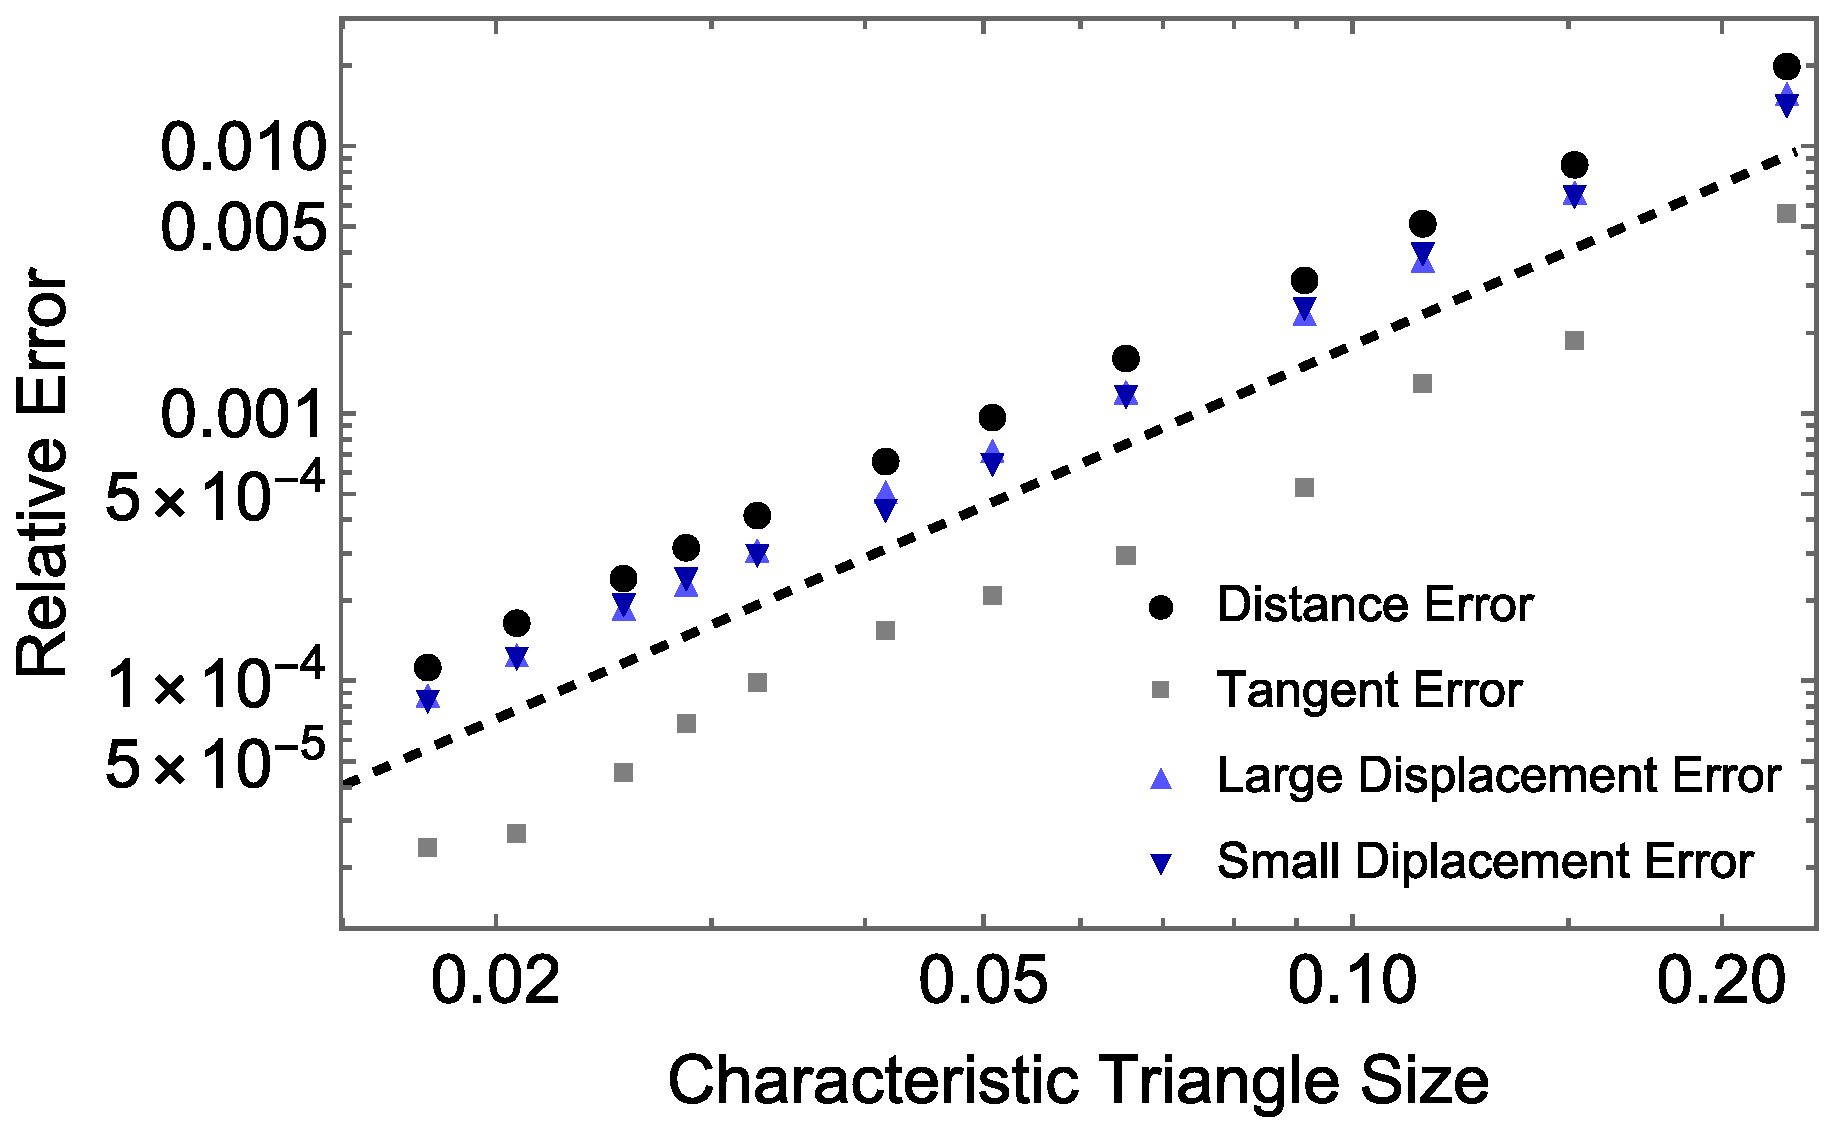
\includegraphics[width=1.0\columnwidth]{error_v_trisize.pdf}
    \caption{Relative error in the geodesic distance (black circles), gradient of the geodesic distance (gray squares), and location after random displacements with large (light blue upward triangle) and small (dark blue downward triangles) magnitdes on a spherical surface of unit radius. Errors are measured against same quantities calculated analytically on a smooth sphere, and we take large and small displacements to correspond to $0.5$ and $0.05$, respectively. Coarser meshes yield less accurate results, and the relative error of all quantities decreases roughly as $h^2$, where $h$ is the square root of the mean triangle area of the corresponding mesh. The dashed line is a guide to the eye with slope 2, and all data points are averages over 200 measurements. }
    \label{fig:error_v_trisize}
\end{figure}


Returning to our simulation framework, the practical calculation of forces reduces to the operation of the \verb+displacement+ algorithm. Given a source particle, we identify all potentially interacting particles as ``targets,'' generate the sequence tree for the source particle, and then query the cached sequence tree to obtain the paths from the source to each of the targets. This gives the lengths $l_{ij}$ and the tangent directions $\dot{\bs{r}}_{ij}$ relative to the source point's location, from which one can (e.g.) compute the total force on $i$ via
\begin{equation}
    F_i = \sum_{j=1}^N{-\frac{dU\left(l_{ij}\right)}{d l_{ij}} \dot{\bs{r}}_{ij}}.
\end{equation}
where the magnitude $\frac{dU\left(l_{ij}\right)}{d l_{ij}}$ is a pre-computed quantity written into a force class. 


For particles interacting via short-ranged forces, this approach contains an obvious inefficiency. The XW algorithm scales with the \emph{total} number of vertices of the discretized surface, but particles may only be interacting in a much smaller local patch of the surface. For short-range interactions, then, we perform a \emph{submeshing} operation: for a potential that vanishes beyond some distance $\sigma$, we exploit the fact that the Euclidean distance between two points is a \emph{lower bound} to the geodesic distance. For a given source particle, we consider the local patch of the surface which contains only those triangular faces (and target particles) whose minimum Euclidean distance is within $\sigma$ of the source particle position, and then build the XW sequence tree only for these local patches. Since the local patch might contain a number of vertices $V' \ll V$, this can speed up the computation of each time step by orders of magnitude. The overarching workflow of distance calculation is depicted in Fig.~\ref{fig:force_flowchart} as an algorithmic flowchart.

\begin{figure}
    \centering
    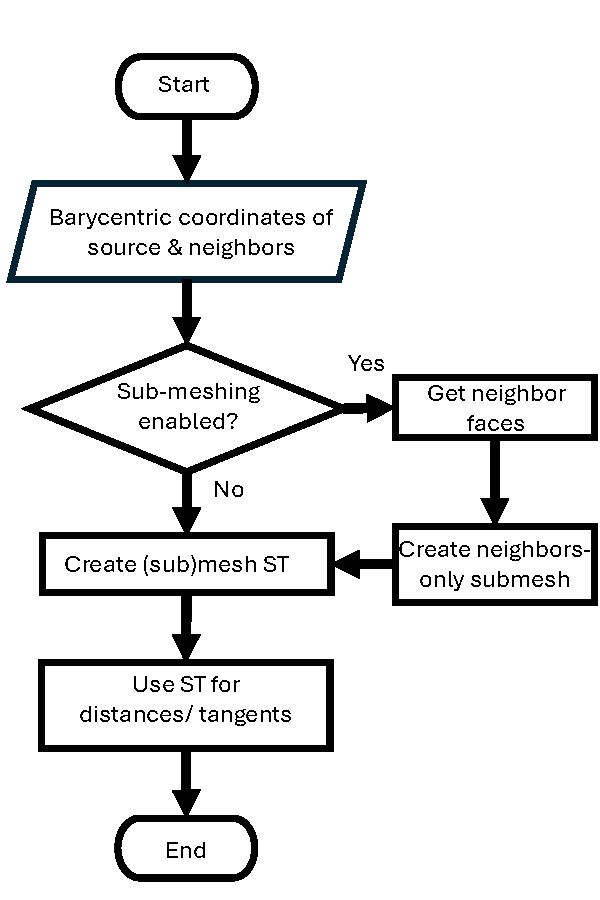
\includegraphics[width=1.0\columnwidth]{force_flowchart_v4.pdf}
    \caption{Depiction of the distance calculation process. The \emph{sequence tree} (ST) is an object which stores information about mesh traversal used in the Xin and Wang algorithm.} 
    \label{fig:force_flowchart}
\end{figure}

\subsection{Updating state information}

The simpler of the two main algorithmic tasks, in flat space and on curved surfaces, is the \verb+shift+ update of positions and velocities of particles given a displacement vector. Force and velocity vectors are \emph{always} defined in the tangent plane of the particle's current face, and we require (a) that all requested displacements are likewise in the tangent plane and (b) that at all times the particles remain on the surface. One strategy for achieving this goal is to use a projection operator approach: for instance, a particle would be displaced by $\bs{d}$ via standard vector addition (which is, indeed, the entirety of the \verb+shift+ algorithm in flat space), and then projected back to the nearest point on the discretized surface. While straightforward, this leads to displacements that do not themselves follow geodesics -- i.e., they are not the equivalent of a ``straight'' displacement.

\begin{figure}[th]
    \centering
    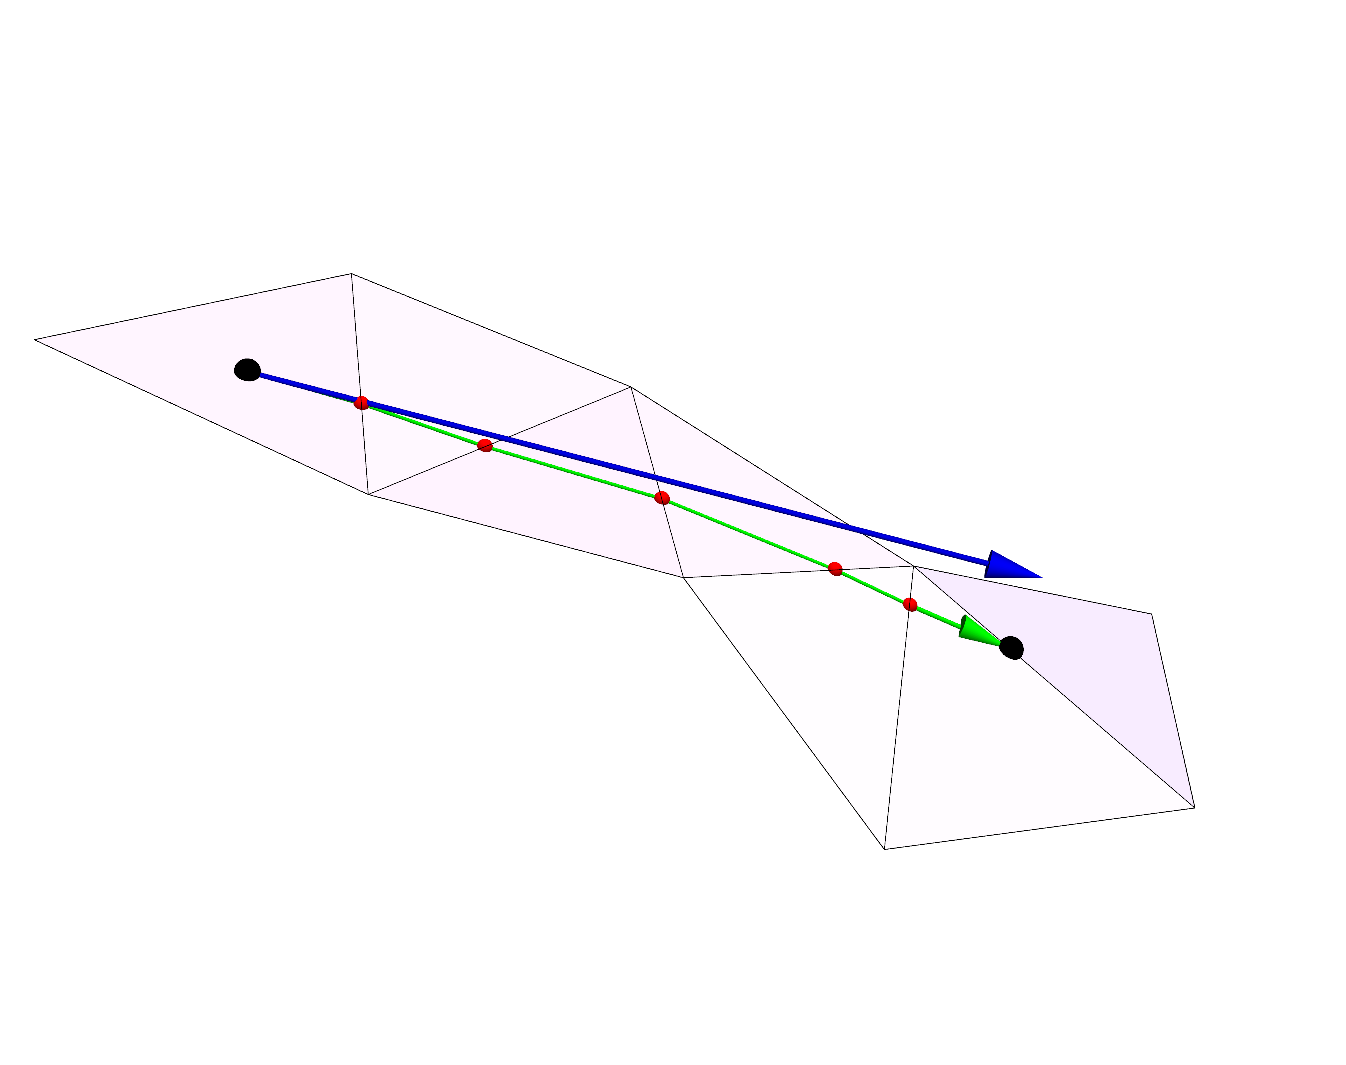
\includegraphics[width = 1.0\columnwidth]{path_rotate_2.pdf}
    \caption{Operation of the \texttt{shift} algorithm: an initial position, marked by the left-most large black point, is moved by a target displacement of direction and magnitude indicated by the blue arrow. The in-surface green arrow represents the progressive rotation of the displacement vector around intersected edges in order to follow a discrete geodesic, which terminates at the right-most large right-most black point. Intersections between the path and the edges are marked by smaller red points. In-face displacements and rotations around edges continue until the total target displacement has been achieved.}
    \label{fig:wraparound_shift}
\end{figure}

Instead, we move across connected faces along a path whose total length is the same as the magnitude of the desired initial displacement. Every time an edge is crossed, the path is rotated around the axis defined by the cross product of the face normals, as shown in Fig.~\ref{fig:wraparound_shift}. This is equivalent to first defining a vector corresponding to the direction and magnitude of desired motion and then unfolding a sequence of faces so that the vector corresponds to a straight line that stays entirely within a connected set of faces -- i.e., of shifting the particle along  a geodesic.
The only ambiguity occurs when a vector would pass through a spherical vertex ---that is, a vertex for which the sum of edge-edge angles is less than $2\pi$.
Here the straightest path (which continues through the vertex) is no longer the shortest path on the surface (which does not). The physical choice in such a case is to displace particles along the straightest-but-not-shortest path, which corresponds to maintaining (e.g.) the direction of particle velocity \cite{polthier2006straightest}.


\begin{figure}[t]
    \centering
    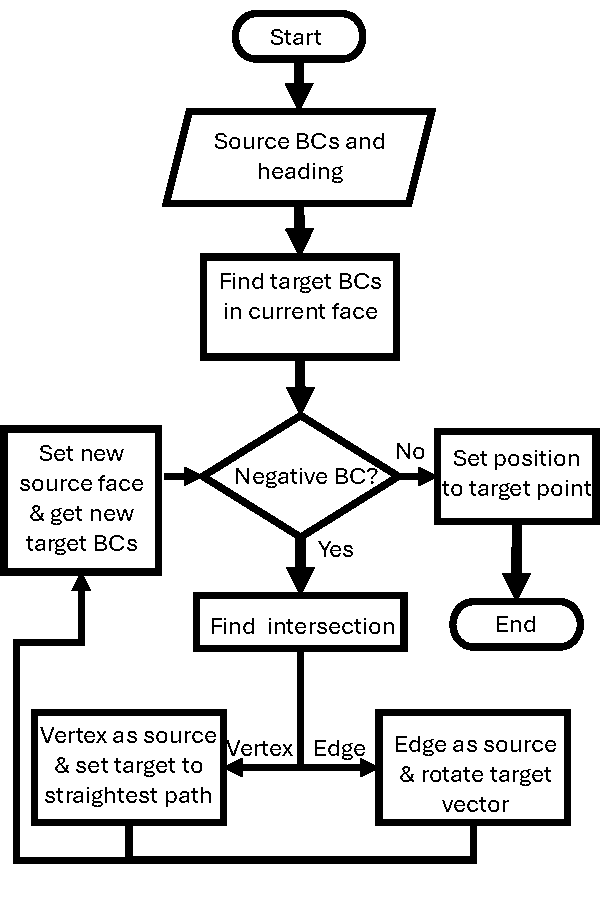
\includegraphics[width=1.0\columnwidth]{shift_flowchart_v4.pdf}
    \caption{Depiction of the shift process, where BC stands for ``barycentric coordinates.'' As described in the main text, how target or parallel transported vectors are rotated depends on whether the intersection is with an edge or a vertex.}
    \label{fig:shift_flowchart}
\end{figure}

Because it is not \emph{a priori} clear given a point and a displacement vector how many faces will be crossed, in our \verb+shift+ algorithm we implement a while loop that (a) checks for intersections --- in barycentric coordinates, to minimize finite-precision issues in these geometrical calculations --- between a  ray emanating from the  particle's current location and any edge of its current face, (b) moves the particle along that vector to either the final location (if in the face) or the intersection point, (c) if necessary, updates the face associated with the particle to the face that shares the intersected edge with the original face, and (d) rotates the vector about the intersected edge into the plane of the new face. This procedure is repeated until a total displacement of the correct magnitude has been performed (with appropriate cases handling intersections with vertices rather than edges). This loop has the benefit of also easily handling parallel transport of vectors as well as shifts of particle positions: a velocity or force vector simply gets carried along with the position, rotating along with the rotation of the displacement vector  as edges or vertices are crossed. Figure \ref{fig:shift_flowchart} depicts the \verb+shift+ routine as an algorithmic flowchart, and its accuracy as a function of mesh discretization is shown for spherical meshes in Fig.~\ref{fig:error_v_trisize}.


\section{Performance Benchmarks}\label{sec:benchmarks}

For all single-core simulations we benchmarked our simulation architecture on a Dell OptiPlex 7080 workstation with an Intel
i9-10900K CPU clocked at 3.70 GHz. All benchmarking and example simulations were done using a single thread, except where noted otherwise; where used MPI benchmarks were conducted on the NCSA Delta CPU cluster using AMD EPYC 7763 processors. 


We first test the performance of our algorithm on a fixed surface at fixed discretization scale (in this case, a torus with minor radius $r_1=1$ and major radius $r_2=3$, discretized into $4616$ triangular faces), as a function of the number of particles, $N$. For the main test we considered a finite-range repulsive pairwise potential whose interaction range was set to $\sigma=1$, and we computed the mean time to execute a timestep of velocity Verlet dynamics. For a standard (flat space) simulation \emph{at fixed density} one would expect $\mathcal{O}(N \log N)$ scaling; in a domain of fixed spatial extent the number of interacting particle pairs itself grows with $N$, and we would anticipate  roughly $\mathcal{O}(N^{1.5})$ scaling for particles that attempt to uniformly cover the curved surface. This is roughly consistent with the observed scaling shown in Fig.~\ref{fig:computationalComplexityFixedMesh}.

\begin{figure}[th!]
    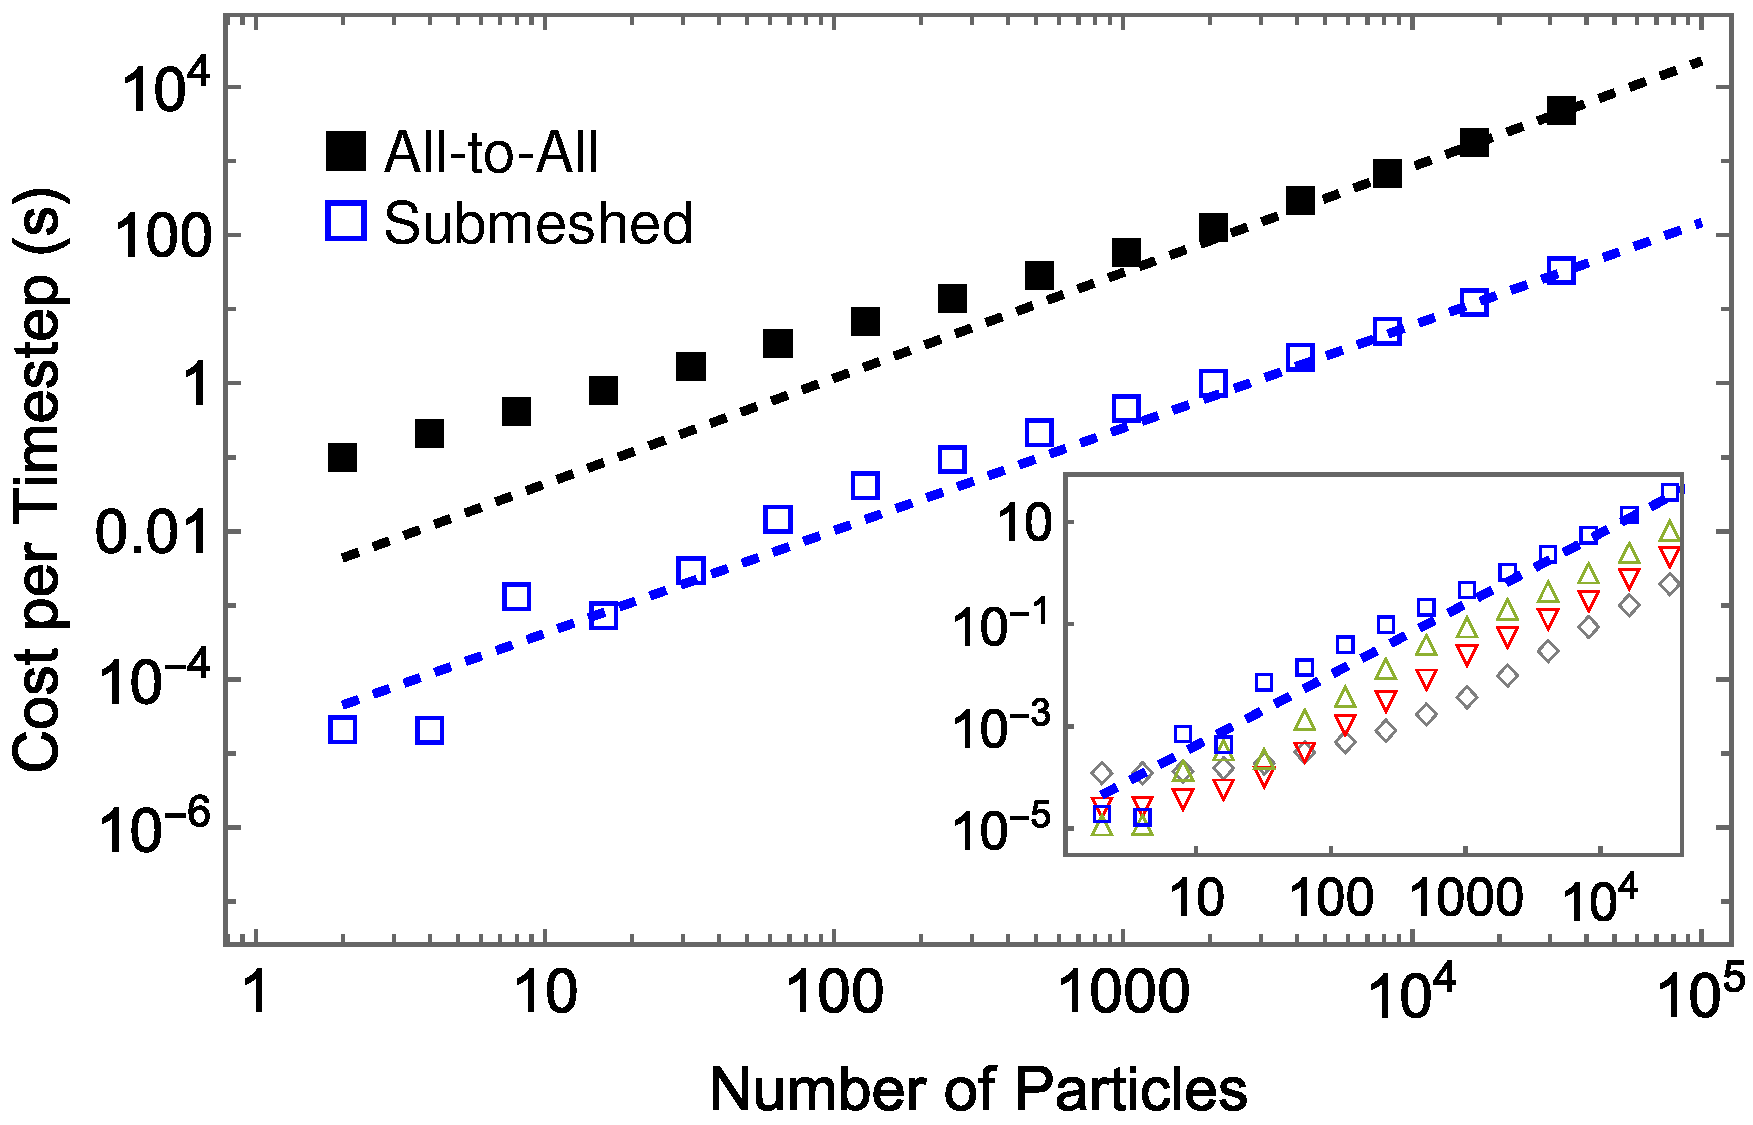
\includegraphics[width=\columnwidth]{pretty_cvn_8_27_fitted.pdf}
    \includegraphics[width=\columnwidth]{strongscaling.png}
    \caption{Simulation cost on a fixed (toroidal) mesh. (Top) The main figure shows the time per time step for a velocity Verlet timestep as a function of the number of particles on the surface. The filled  black squares correspond to calculating sequence trees for the entire mesh, whereas the open blue squares correspond to using a submesh scale of $\sigma=1$. Lines reflect fits to the asymptotic behavior of the two strategies, which both behave as power laws with scaling exponent approximately $1.4$. The inset shows the simulation cost as a function of varying $\sigma$. From top to bottom the symbols correspond to $\sigma = 2^{-n}$ for $n=0,1,2,3$, with the dashed line from the main image reproduced for convenient comparison. (Bottom) Strong scaling analysis of the default MPI implementation, showing the speedup relative to single-core performance as a function of the number of MPI ranks. From light to dark, the total number of simulated particles ranges from $N=128$ to $N=131072$ in powers of 2. This test corresponds to implementing NVE equations of motion on an aspect-ratio 3 torus discretized into 4616 faces using soft particles that interact in a range $\sigma=2^{-3}$. The dashed line is a guide to the eye of slope $-1$, corresponding to ideal strong scaling behavior. The inset shows the raw profiled cost per timestep (in seconds) as a function of MPI ranks for the same data as in the main panel.}
    \label{fig:computationalComplexityFixedMesh}
\end{figure}

We also have implemented a basic MPI communication pattern using the openMPI framework \cite{gabriel2004open} pattern to partition work across multiple processors -- for our basic implementation we note that the cost of computing even submeshed sequence trees is substantially higher than the cost of the mere vector addition and subtraction needed to compute distances and gradients in flat space, and we expect large gains from parallelization by arbitrarily and evenly dividing the cost of computing forces on particles among the available processors. A future enhancement to this would involve further using spatial location of the particles to divide the computational workload, as is common in  molecular dynamics in flat space. Nevertheless, we observe reasonable strong scaling behavior of our simple implementation at modest system sizes. We test our implementation by choosing a fixed mesh (a torus whose large radius is 3 in simulation units, small radius is 1, discretized into 4616 faces) and investigating the time to complete NVE timesteps relative to a single-core simulation for varying numbers of particles and CPU cores. The bottom panel of Fig. \ref{fig:computationalComplexityFixedMesh} shows the speedup (defined as the profiled time per timestep when running on a single MPI rank divided by profiled time per timestep when running on multiple ranks) for particles interacting via a soft harmonic potential of range $\sigma=1/8$. For this naive implementation, we estimate that assigning we estimate that assigning each processor of order $2\times 10^3$ particles almost completely hides the communication cost and results in ideal strong scaling. For particles interacting with greater range, we expect that a correspondingly smaller number of particles per processor would hide the communication cost.

The counterpart to these  analyses is to consider simulating a fixed  number of particles on meshes of increasing numbers of vertices -- this corresponds to the spatial version of choosing a time-step size that sufficiently minimizes discretization error. In addition to the $\mathcal{O}(V^2 \log V)$ worst case scaling for building the sequence tree, there are also geometric prefactors (the length scale of curvature variations, the density and placement of saddle vertices, etc) that can strongly influence the cost of these calculations. Some benchmarks have even reported non-monotonic scaling in the sequence tree generation time as a function of vertex number in some regimes \cite{cgalklcdvtsmsp23b}. In Fig.~\ref{fig:computationalComplexityFixedParticleNumber}  we report the mean time to complete a timestep as a function of  $V$ for a small number of  representative surfaces: a sphere (for which all calculations  can be compared with the analytical result), tori of two different aspect ratios (3 and 20), and an elephant (in this case, represented as a geometrically interesting genus-3 surface). In all of these tests we hold the mesh span and the range of interactions fixed while 
increasing the number of triangles used to discretize the surface with an incremental triangle-based isotropic remeshing algorithm \cite{botsch2004remeshing}. We indeed find experimentally that there can be important differences when simulating particles on different meshes. Reflecting the local flattening that submeshing can accomplish, we find very roughly $\mathcal{O}(V^{1.5})$ scaling for finite-range simulations compared to roughly $\mathcal{O}(V^{2})$ behavior for computing sequence trees across the entire mesh.


\begin{figure}[hbt]
\centering
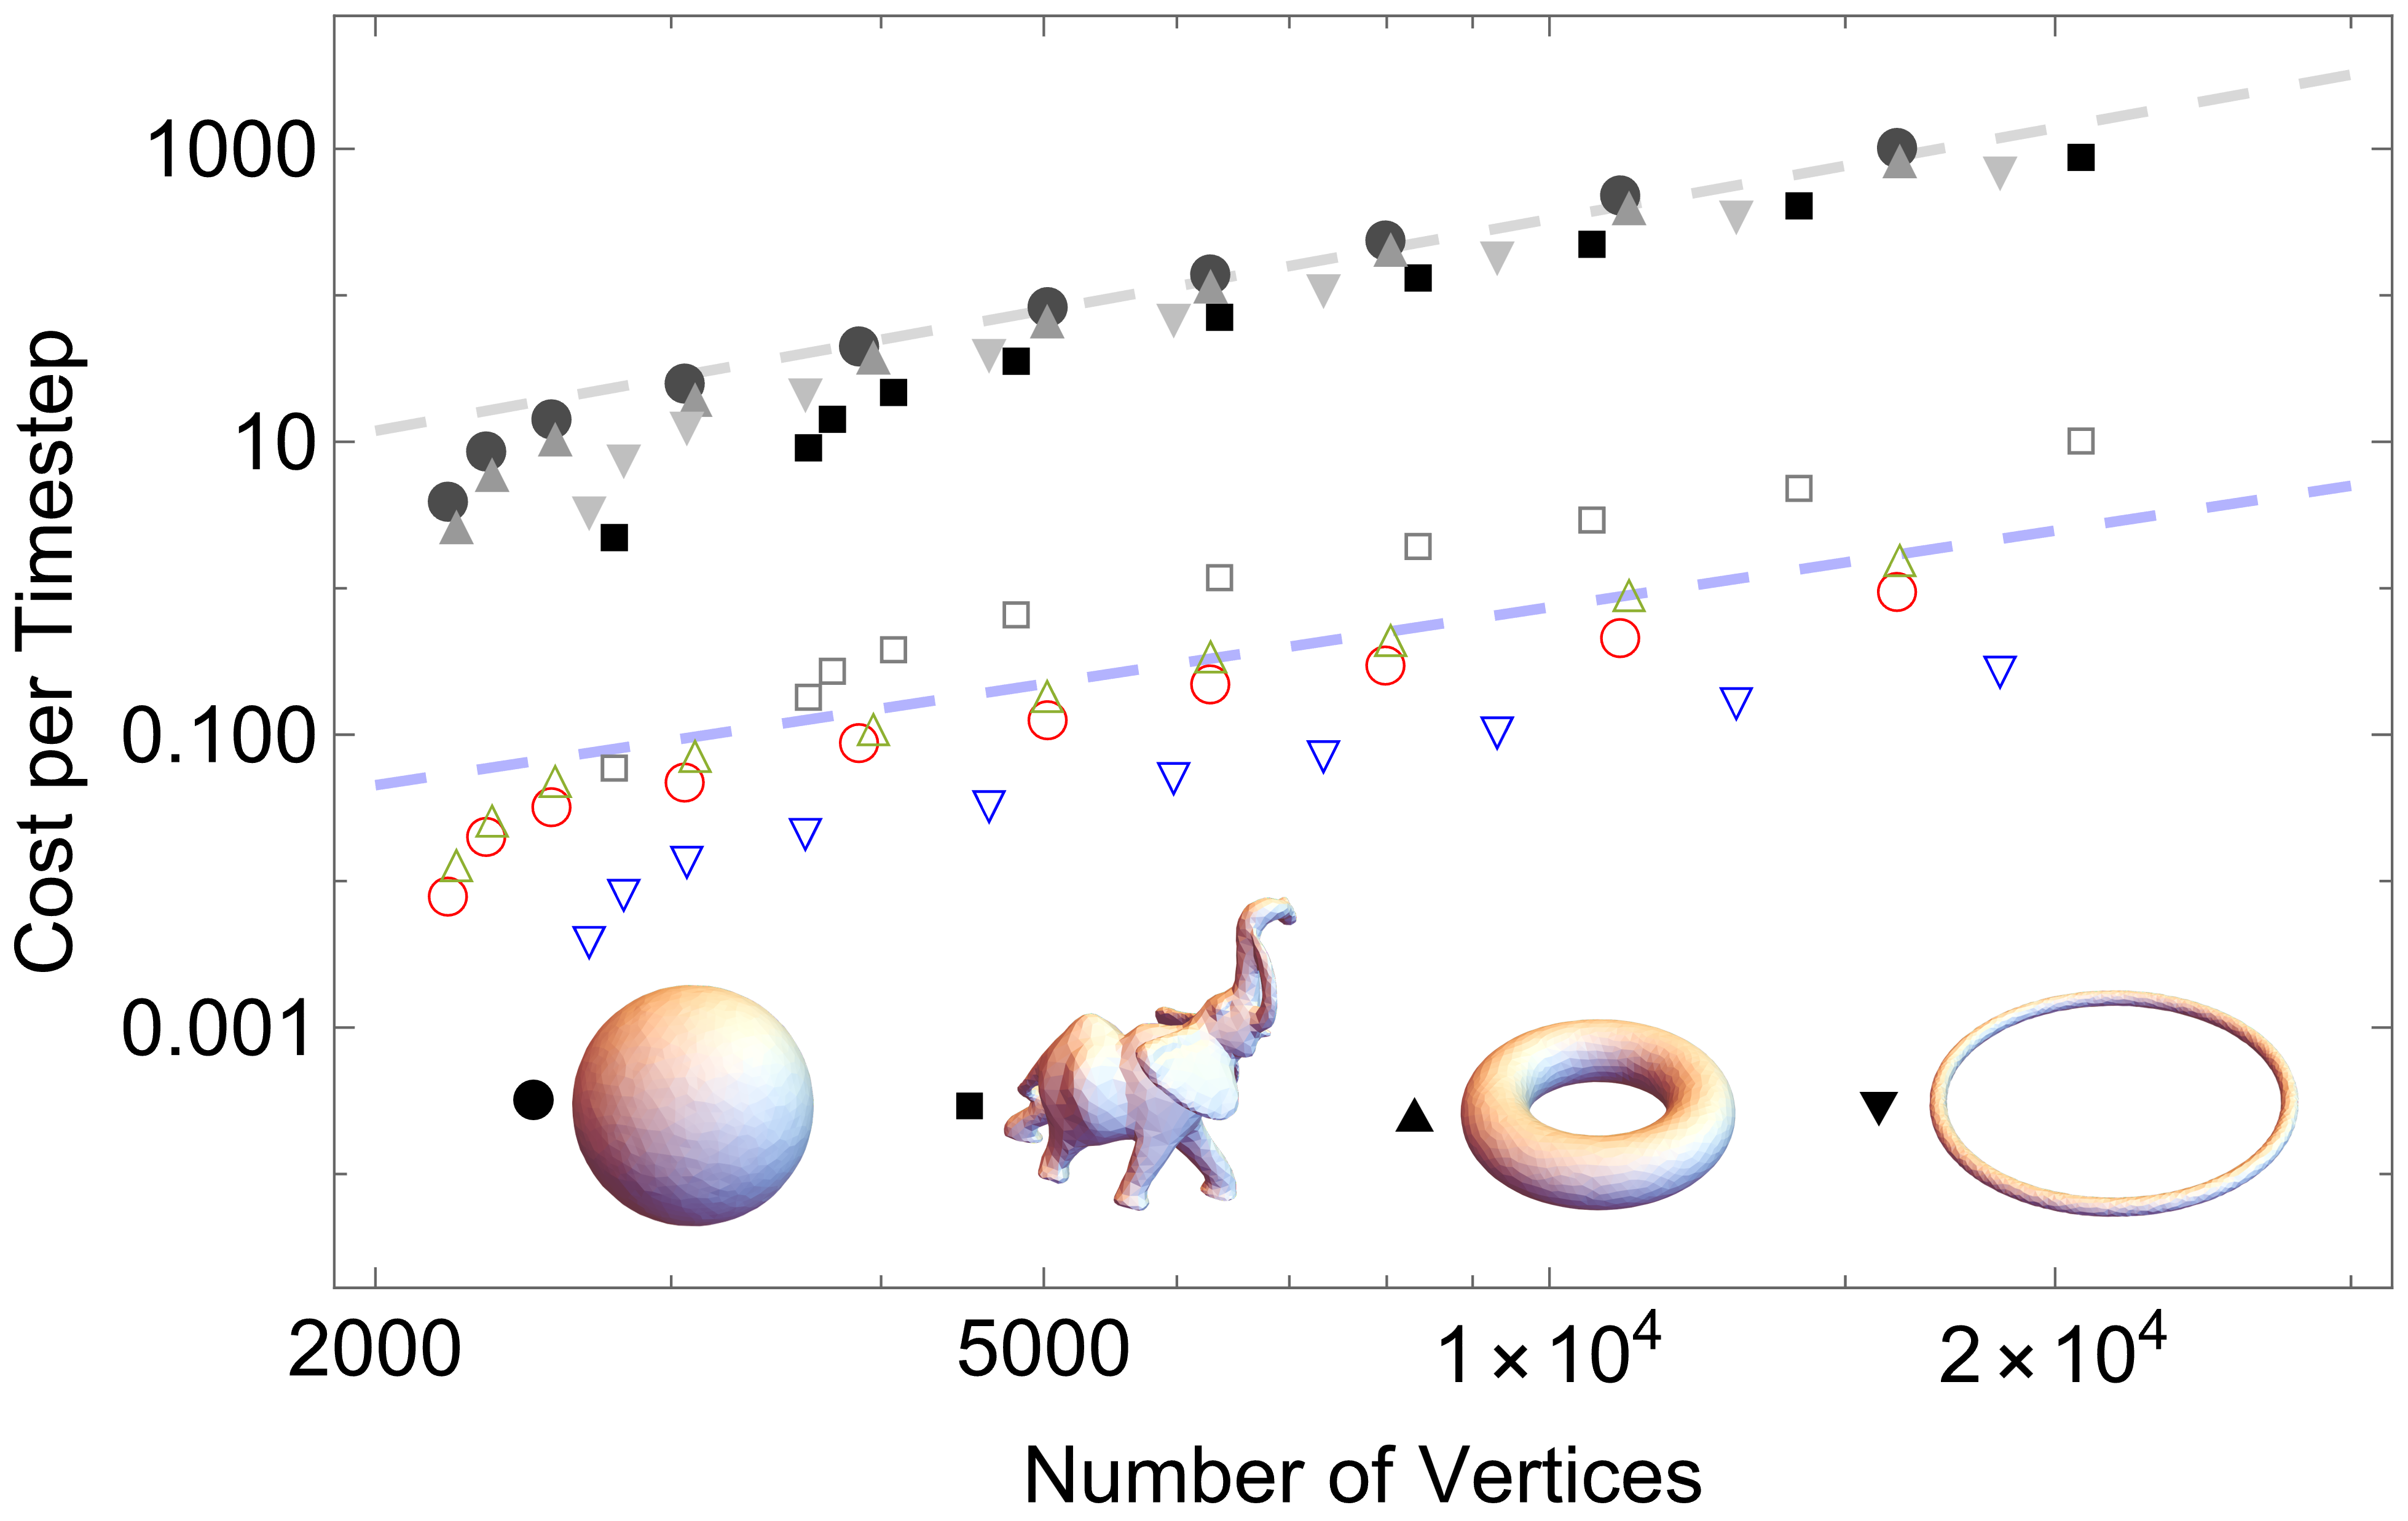
\includegraphics[width=\columnwidth]{cvc_final_spread_meshes.png}
\caption{Mean time per NVE timestep for $N=100$ particles on four surfaces upon isotropically increasing the number of vertices in each mesh. Solid symbols correspond to calculating sequence trees over the entire mesh for every particle, and open symbols correspond to using our submeshing routines for interactions of fixed range. For all surfaces, we chose an interaction range corresponding to one-tenth of the total span of the mesh in order to fairly compare across very different surface geometries.
The upper dashed line has slope $m\approx 2.07$, while the lower line has slope $m\approx 1.73$; each is an approximate fit to the the aspect-ratio-3 torus data.}
\label{fig:computationalComplexityFixedParticleNumber}
\end{figure}


\section{Crystallization on the surface of a torus}\label{sec:example}

In this section and the next we present two examples in which we study ground-state configurations of particles on curved surfaces and compare with some results in the literature. Here, we first consider particles interacting via purely repulsive potentials on the surface of the torus.
The torus is often taken as one of the simplest examples of a topologically non-trivial surface with gradients in the surface curvature \cite{bowick2009two}, and crystallization on their surface has been studied both theoretically and numerically \cite{giomi2008elastic,giomi2008defective}. We make some direct comparisons with those earlier numerical studies, which implemented with forces between particles according to Euclidean (rather than geodesic) distance and used a long-range Riesz potential ($U(l_{ij}) = l_{ij}^{-3}$) to ensure that in ground states particle positions were on the surface of the torus.

\begin{figure}[b!]
\centering
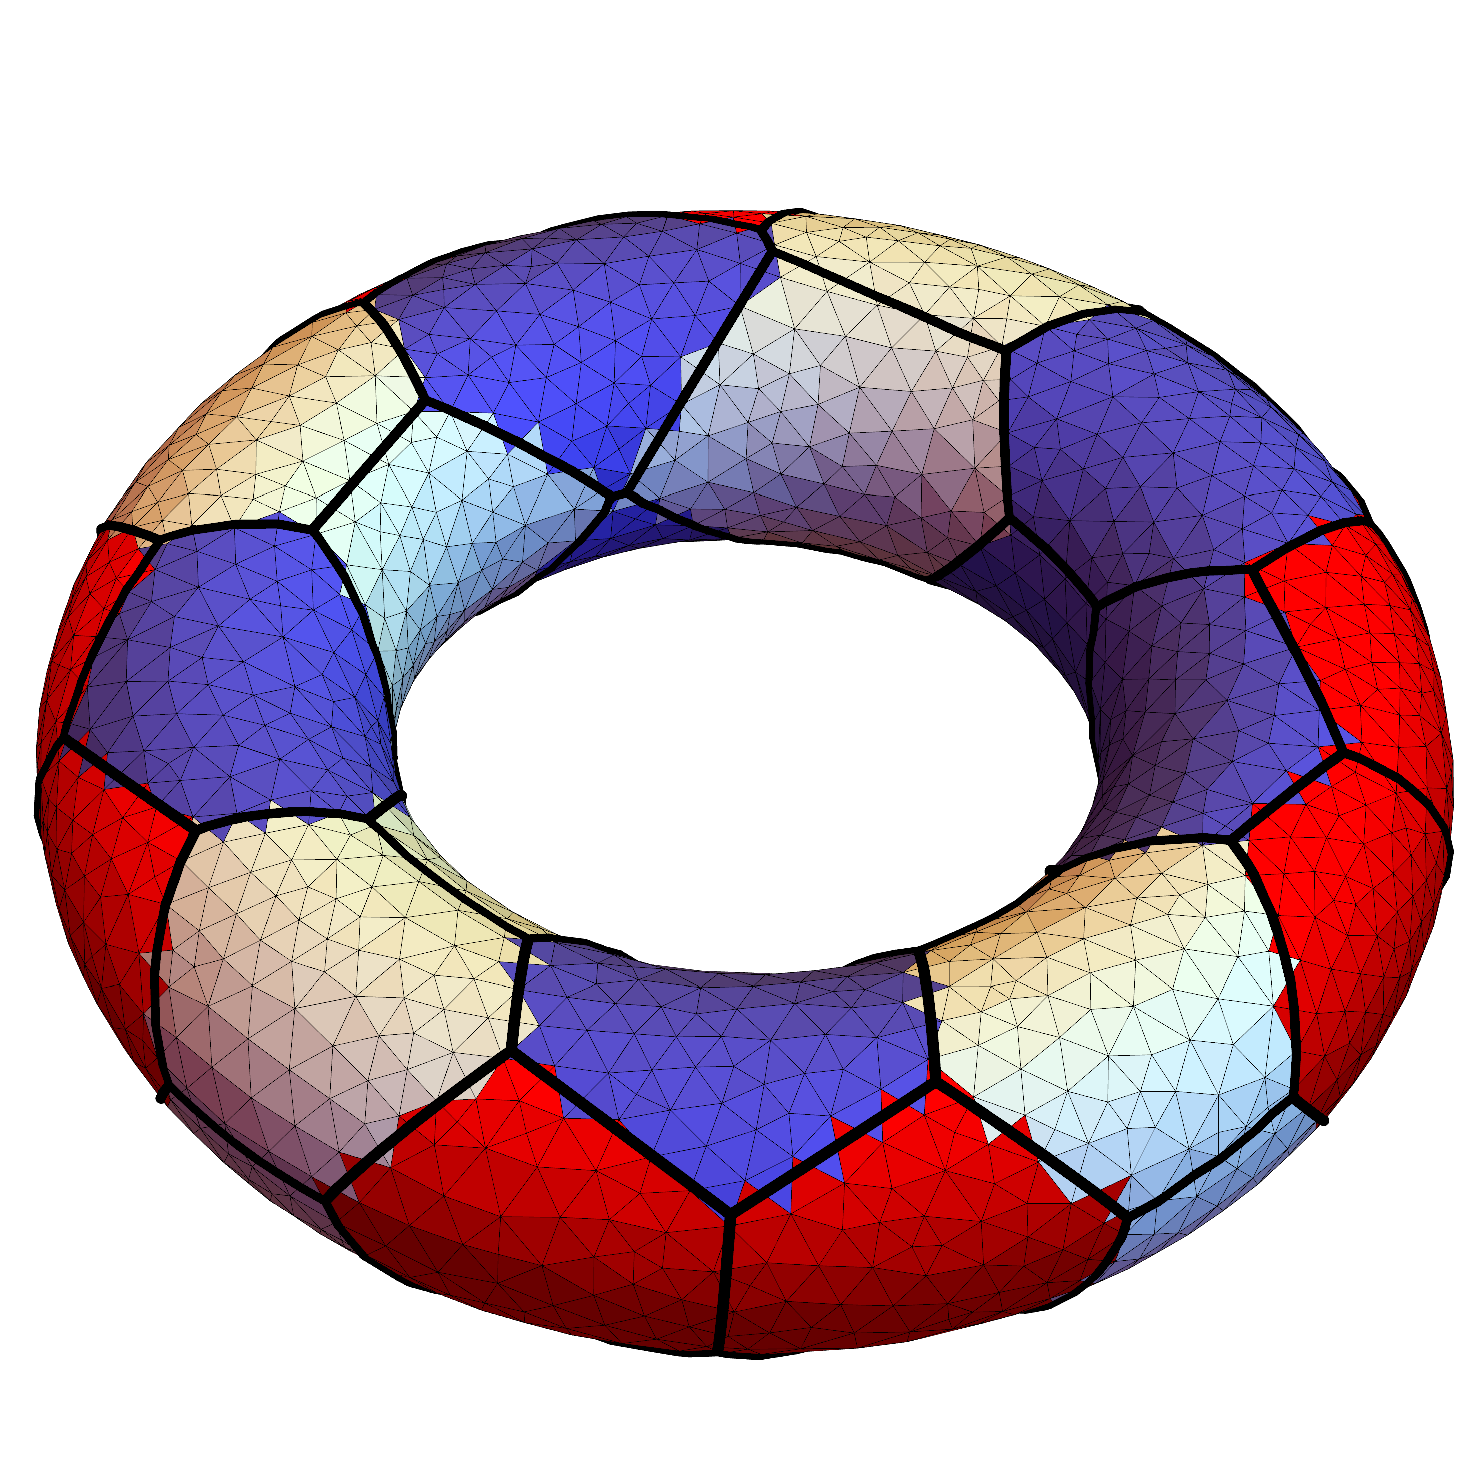
\includegraphics[width=0.75\columnwidth]{32_particle_voronoi_regions.pdf}
\caption{The Voronoi diagram of a 32-particle local energy minima on the surface of the torus found via gradient descent. The boundaries of the Voronoi regions are shown with thick black lines, and the triangles of the underlying mesh are colored according to the connectivity of the particle nearest to their centroid in the surface Voronoi diagram: red regions correspond to particles with five neighbors, blue to particles with seven, and white to particles with six. The ground state found here has 10 five-seven defect pairs, whereas the ground state configuration predicted in Ref.~\cite{giomi2008elastic} has 16 five-seven defect pairs.}
\label{fig:smallTorusSmallNConfiguration}
\end{figure}

Ref.~\cite{giomi2008elastic} predicts a variety of interesting toroidal crystals -- these range from precise ground state configurations in the small-$N$ regime, to patterns of crystalline defects, to limiting torus aspect ratios beyond which defect-free configurations should be the true ground state of the system. In Fig.~\ref{fig:smallTorusSmallNConfiguration} we show an in-surface Voronoi diagram (generated as a restricted Euclidean Voronoi diagram via SurfaceVoronoi \cite{xin2022surfacevoronoi}) of a typical low-energy configuration. 

As gradient descent is particularly suitable for finding nearby \emph{local} minima rather than global minima, in the tests below we primarily aim to find expected distributions of defects and qualitative geometric signatures, rather than true ground states. For example, given 32 particles on an aspect ratio 3 torus, the true ground state consists of 16 pairs of 5-7 defects -- 16 particles with 5 neighbors and 16 particles with 7 neighbors -- arranged on the outer and inner portions of the torus, respectively \cite{giomi2008elastic}. While gradient descent starting from a random point pattern does not find the true ground state, we indeed find a set of defect pairs distributed in the expected regions of the torus, as seen in  Fig.~\ref{fig:smallTorusSmallNConfiguration}. 


\begin{figure}[b!]
\centering
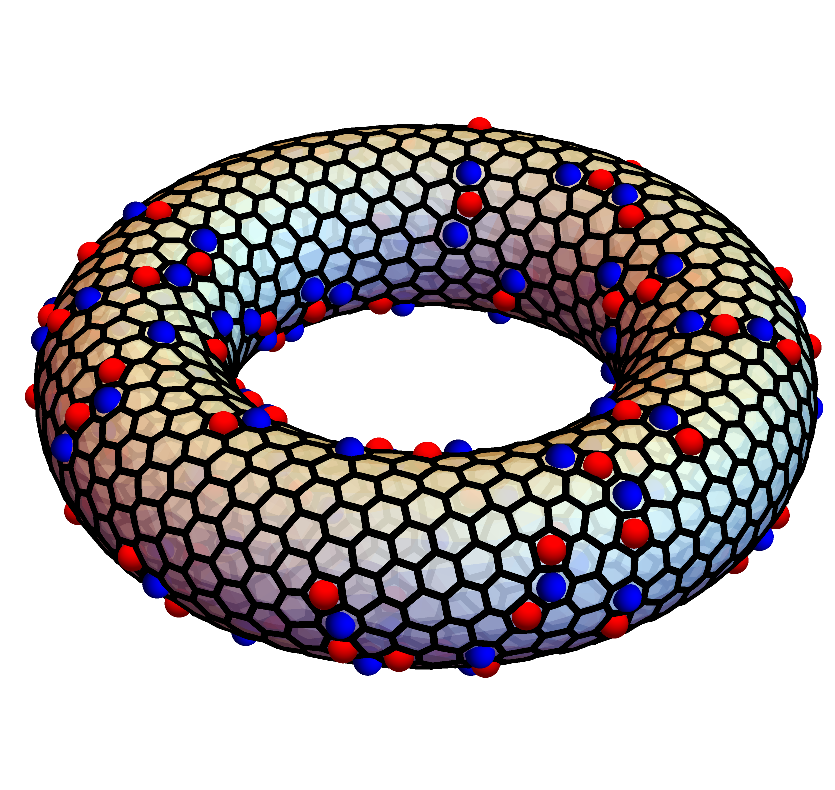
\includegraphics[width=0.75\columnwidth]{1000_particle_voronoi_points.pdf}
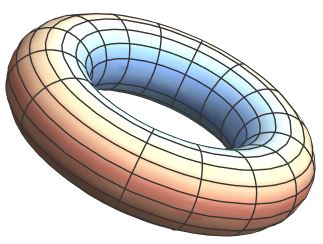
\includegraphics[width=0.75\columnwidth]{torusDefectHeatmap.JPG}
\caption{ (Top) A relaxed configuration of 1000 particles on the surface of a torus. Here, rather than a strict localization of five-fold and seven-fold defects to the outer and inner equators of the torus as expected in the true ground state, we observe chains of defects populating the surface. This is expected from the elastic theory (described in more detail in \cite{giomi2008elastic}), from which we expect that larger particle numbers cause the amount of curvature required to screen defects from each other to be so large that defect chains, or ``scars,'' develop. (Bottom) A heat map indicating the average net defect charge across the surface (with red corresponding to an excess of five-fold defects and blue to an excess of seven-fold defects) over 1000 quenches of an $N=500$ particle configuration. Again, the correlation between the spatial distribution of Gaussian curvature and defect distribution is as expected.}
\label{fig:smallTorusLargeN}
\end{figure}

As the number of particles on the surface of the torus increases, we expect to find \emph{chains} of defects coexisting with a large number of particles which interact with six neighbors \cite{giomi2008elastic}. We performed an $N=1000$ particle simulation which began from a random initial distribution of positions and relaxed via gradient descent. We observe a greater total number of defects than expected in the true ground state \cite{giomi2008elastic}, but as shown in the top panel of Fig.~\ref{fig:smallTorusLargeN} we indeed found the the qualitatively expected result that in this particle-number regime defects are primarily localized along chains. Leveraging the computational efficiency afforded by our simulation framework, we performed over 1000 separate energy minimizations of $N=500$ particles to find the expected distribution of defect charge in these local energy minima. As seen in the bottom panel of Fig.~\ref{fig:smallTorusLargeN}, we find that (as expected) there tend to be excesses of 7-fold and 5-fold defects on the inner and outer portions of the torus, and where the Gaussian curvature vanishes, so too does the expected defect charge.


For tori of larger aspect ratio, the ground states correspond to lattices with a slow twist -- particles forming helical chains around the surface -- but fewer total defects. We initially seed 300 particles positions on an aspect-ratio-20 torus on a lattice with \emph{incommensurate} twist (so that the initial configuration, while not disordered, is nevertheless far from the true ground state). We find that the particles relax to a structure with regions of correct crystalline order separated by grain boundaries. This is shown in Fig.~\ref{fig:largeTorusConfigurationComparison}. 
In detail, this configuration has 11 five-fold and seven-fold defects, many localized between different twisted lattice configurations (e.g., on the top left of the figure).

\begin{figure}[htb!]
\centering
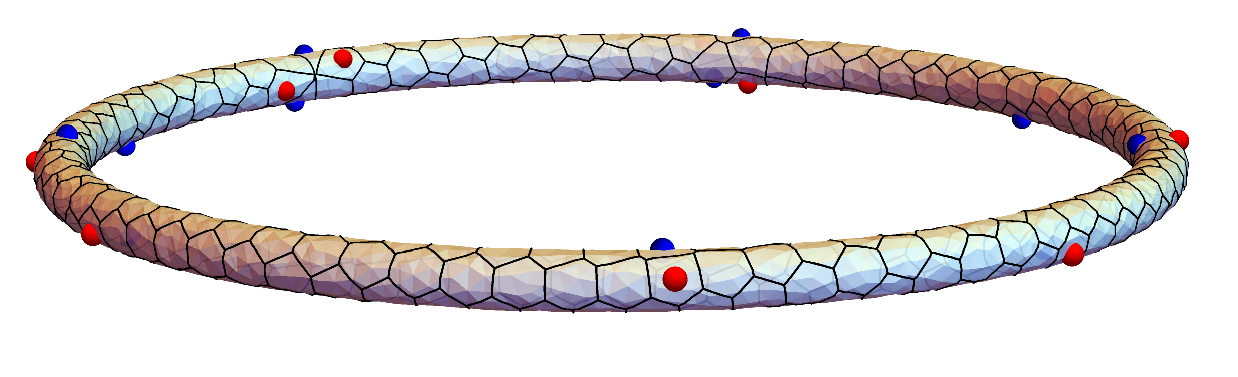
\includegraphics[width=1\columnwidth]{300_big_particle_voronoi_points.pdf}
\caption{A low-energy configuration of $N=300$ particles on a narrow (aspect ratio 20) torus. While gradient descent does not easily find the defectless ground state, this local minimum has relatively low defect number (11 five-fold and seven-fold defects, denoted with red and blue points, respectively).}
\label{fig:largeTorusConfigurationComparison}
\end{figure}

We have included supplemental videos showing the evolution of particle positions during minimization corresponding to the results shown in Figs.~\ref{fig:smallTorusSmallNConfiguration}-\ref{fig:largeTorusConfigurationComparison}. We have shown that we can reproduce qualitatively expected signatures of ground state configurations using direct gradient descent. This includes signatures of the high-defect-number ground state for 32 particles in their relaxed distributions on an aspect ratio 3 torus, defect chains and  expected distributions of defects over multiple quenches for many more particles on the same, and finally twisted regions within the aspect ratio 20 torus that reflect the expected helical configuration in the defectless ground state. Although not our goal in this section, we fully expect that implementing more sophisticated minimization protocols -- simulated annealing, quench-and-perturb, etc. -- would allow us to more fully reproduce the true ground-state behavior reported in the literature \cite{giomi2008elastic}. 

\section{Geometric Configurations on a Filament Bundle-Analogous Surface} \label{sec:example2}

While the toroidal surfaces considered in the previous section are more complex than spherical geometries, we also highlight here our framework's ability to study more complex surfaces --- in this case, by including non-trivial boundary conditions.
To that end, we show numerical results that are complementary to the data on the ground-state configurations of twisted filament bundles in Ref.~\cite{bruss2012non}.
In that work, the filament bundles are characterized by a rate of helical rotation, $\Omega$, about the $z$-axis.
The centerline of a filament  with position $\bs{x}=(x,y)$ at $z=0$ is given by
\begin{equation}
    \bs{r}(\bs{x},z) = \bs{x} \cos(\Omega z) + (\hat{z} \times \bs{x}) \sin(\Omega z) + z \hat{z},
\end{equation}
which is then conveniently rewritten in polar coordinates for which $\rho$ is the radial coordinate and $\phi$ the angular coordinate. Bruss and Grason work out \cite{bruss2012non} the geometry of the vector of closest approach between two filaments as a function of the centerline position in the plane. In the limit of infinitesimal separation, this is
\begin{equation}\label{eq:siloMetric}
   ds^2 = (\delta\rho)^2 + \Omega^{-2}\sin^{2}{\theta(\rho)}(\delta\phi)^2, 
\end{equation}
where 
\begin{equation}
    \theta(\rho) = \arctan\left(\Omega\rho\right)
\end{equation}
is the local tilt angle of a filament. 

Bruss and Grason note that the metric properties of bundle packing can then be understood by actually constructing surfaces that have the metric of Eq.~\ref{eq:siloMetric}, embedding those surfaces in 3D space, and studying disk packings on them.
The authors describe these surfaces as \emph{silo-like}, with a hemispherical cap smoothly transitioning to a cylindrical regime.
An example of such a surface is depicted in Fig.~\ref{fig:siloMeshPicture}.

\begin{figure}
    \centering
    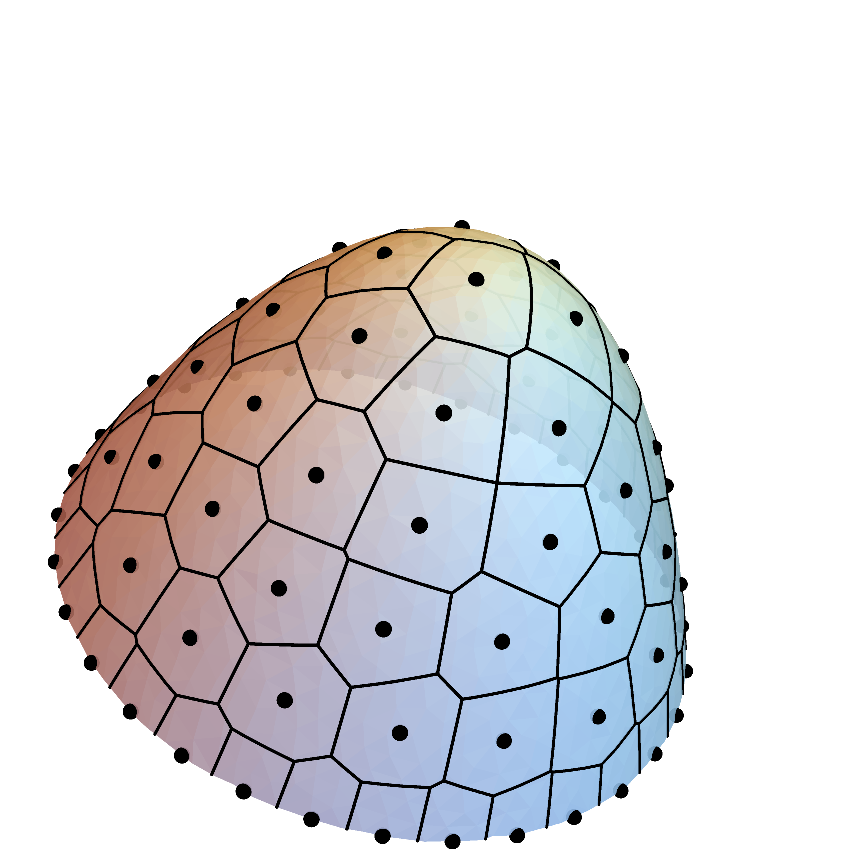
\includegraphics[width=1.0\linewidth]{82_omega028_18.pdf}
\caption{A representation of the surface implied by Eq.~\ref{eq:siloMetric}, here with $\Omega=0.028$. A minimized configuration of particles interacting via soft harmonic repulsion is shown, together with the geodesic Voronoi diagram corresponding to that configuration.}
    \label{fig:siloMeshPicture}
\end{figure}

Previous work in Ref.~\cite{bruss2012non} includes both asymptotic close packing analyses of twisted filament bundles and augmented steepest-descent energy minimizations to attempt to find ground state configurations. In the latter, filaments interact via a Lennard-Jones potential; to deal with the exponential increase in local energy minima, the authors studied increasingly large ensembles as the bundle grew.
Configurations were analyzed by first conformally mapping the filament coordinates to the 2D plane and performing a standard Delaunay triangulation.
Notable numerical findings include that (a) for finite-sized bundles of radius $R$ the total topological charge of disclinations, $Q$ (expressed not fractionally but rather as the deviation of total coordination from $6N$), was a function only of $\Omega R$, and (b) $Q$ monotonically increased from 0 for weakly twisted ($\Omega R \ll 1$) bundles to a maximum topological charge of $Q=6$ in highly twisted bundles. 

We used curvedSpaceSim to study disk packings on these silo-like surfaces not via asymptotic close packing algorithms that start from a hexagonal lattice \cite{bruss2012non}, or by an augmented steepest-descent-plus-tapping algorithm, but rather by simpler minimization protocols starting from many independently initialized particle configurations. Because curvedSpaceSim takes fixed meshes as its input, varying particle number in our simulations at fixed area fraction allows us to investigate different characteristic lengthscales of the bundle width to the particle size, $R/d$, without having to use many copies of meshes of equal $\Omega$ but varying extent.

We performed our energy minimizations using soft harmonic repulsions, in which the geodesic particle diameter $d$ was set to have approximately equal area fraction $f=0.93$ for different particle number $N$, $d = 2\sqrt{f\frac{A}{N\pi}}$.
Initial particle positions were randomized, and we then performed a sequence of minimizations interleaved with high-temperature melting performed in the NVT ensemble by coupling the system to a Nos\'e-Hoover thermostat.
We set a large enough temperature such that the result was functionally equivalent to starting with a new random configuration, but we wanted to document additional functionality of our simulation framework.
Minimizations were done using the FIRE algorithm \cite{bitzek2006structural}, with the configuration recorded after each minimization step. 200 minimizations were performed on each mesh for each of $N=32$, $82$, $124$, and $256$ particles.
We cataloged $\Omega R$ for each configuration, where $R$ is the geodesic cluster radius.
$R$ was measured as the average geodesic arc length from the center of the mesh cap to particle centers at the cluster edge.

We make two comments on our use of surfaces with a boundary rather than the tori of the previous section. The first is that when using such surfaces we must make a choice of boundary conditions for particle displacements and velocities near the boundary.
In this case, we chose to implement boundary conditions that (a) prevent any particle motion beyond the edge of the mesh, (b) set the component of the velocity normal to the boundary to zero for any particle that contacts the boundary, and (c) freely permits particles to slide tangentially along the boundary.

The second is that these boundary conditions correspond to in-principle unbounded fictitious external forces that we allow to act on the particles (corresponding to the effectively hard constraint keeping particles on the surface). Because of this, while we can still search for force-balanced configurations via energy minimization, we choose not to use an energetic criterion to characterize the quality of the minima we find.
Instead, we evaluate the geodesic Voronoi diagram for all of our minimized configurations, count the total topological charge for each diagram, and report charge statistics for all of these configurations (rather than just the best local minima found).
We further explicitly note that in counting topological charge, we exclude particles on the boundary or their neighbors.


Our results on silos of varying $\Omega$ are shown in Figs.~\ref{fig:meanCharge} and \ref{fig:minCharge}. In the statistics of the average charge over all of our configurations, Fig.~\ref{fig:meanCharge}, we unambiguously recover the previously reported monotonic increase of $Q$ with $\Omega R$. This is true for all values of $R/d$, but it is not clear that in these relatively-highly-defective local states of force balance the mean charge is in fact independent of $R/d$ as suggested in Ref.~\cite{bruss2012non}. The charges of the minimally-defective state in each of our 200 minimizations are shown in Fig.~\ref{fig:minCharge}. We note that with our protocol (i.e., melting the configuration rather than gently tapping the boundary particles) it is much harder to find true crystalline ground states, even for relatively modest particle number. We also note that our counting method for $Q$ --- excluding boundary and boundary-neighbor particles --- is especially problematic at low $N$, and can lead to specific configurations with very low or even spuriously negative counts of topological charge.

\begin{figure}
    \centering
    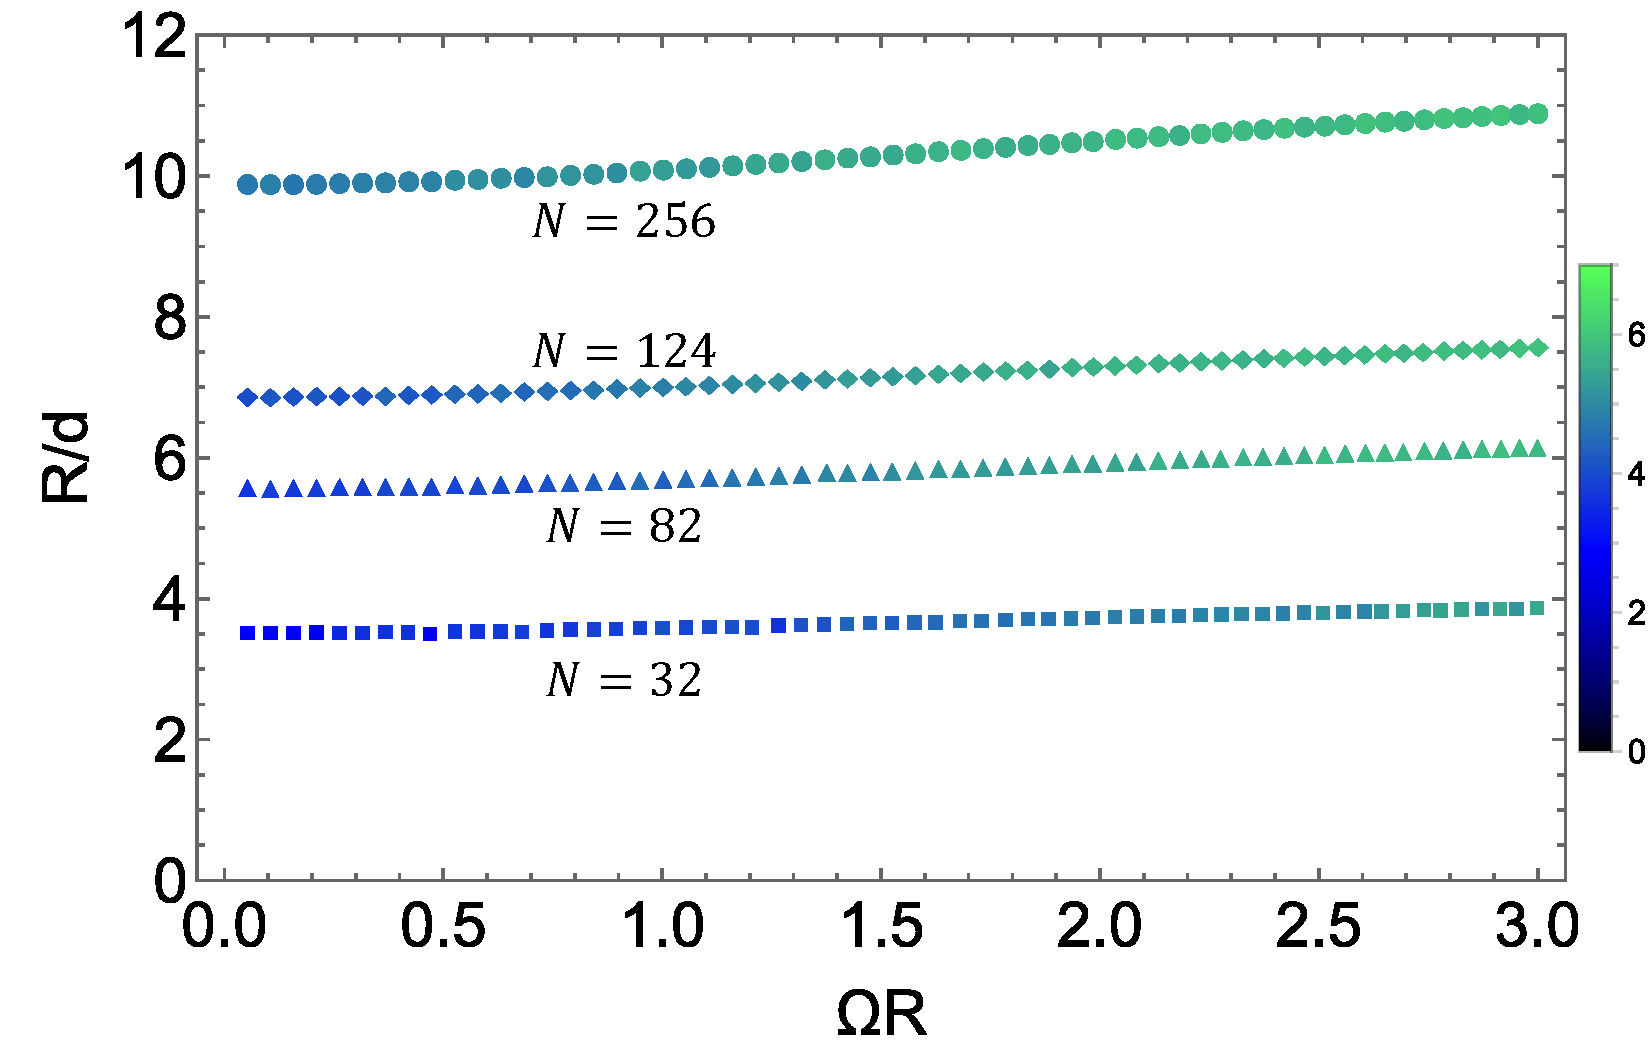
\includegraphics[width=1.0\linewidth]{meancounts_v4.pdf}
    \caption{Mean topological charges $Q$ found for different $R/d$ vs. 
$\Omega R$ represented by a continuous color scale. As $\Omega R$ increases the mean topological charge increases, as does the charge at fixed $\Omega R$ with increasing $R/d$.}
    \label{fig:meanCharge} 
\end{figure}

\begin{figure}
    \centering
    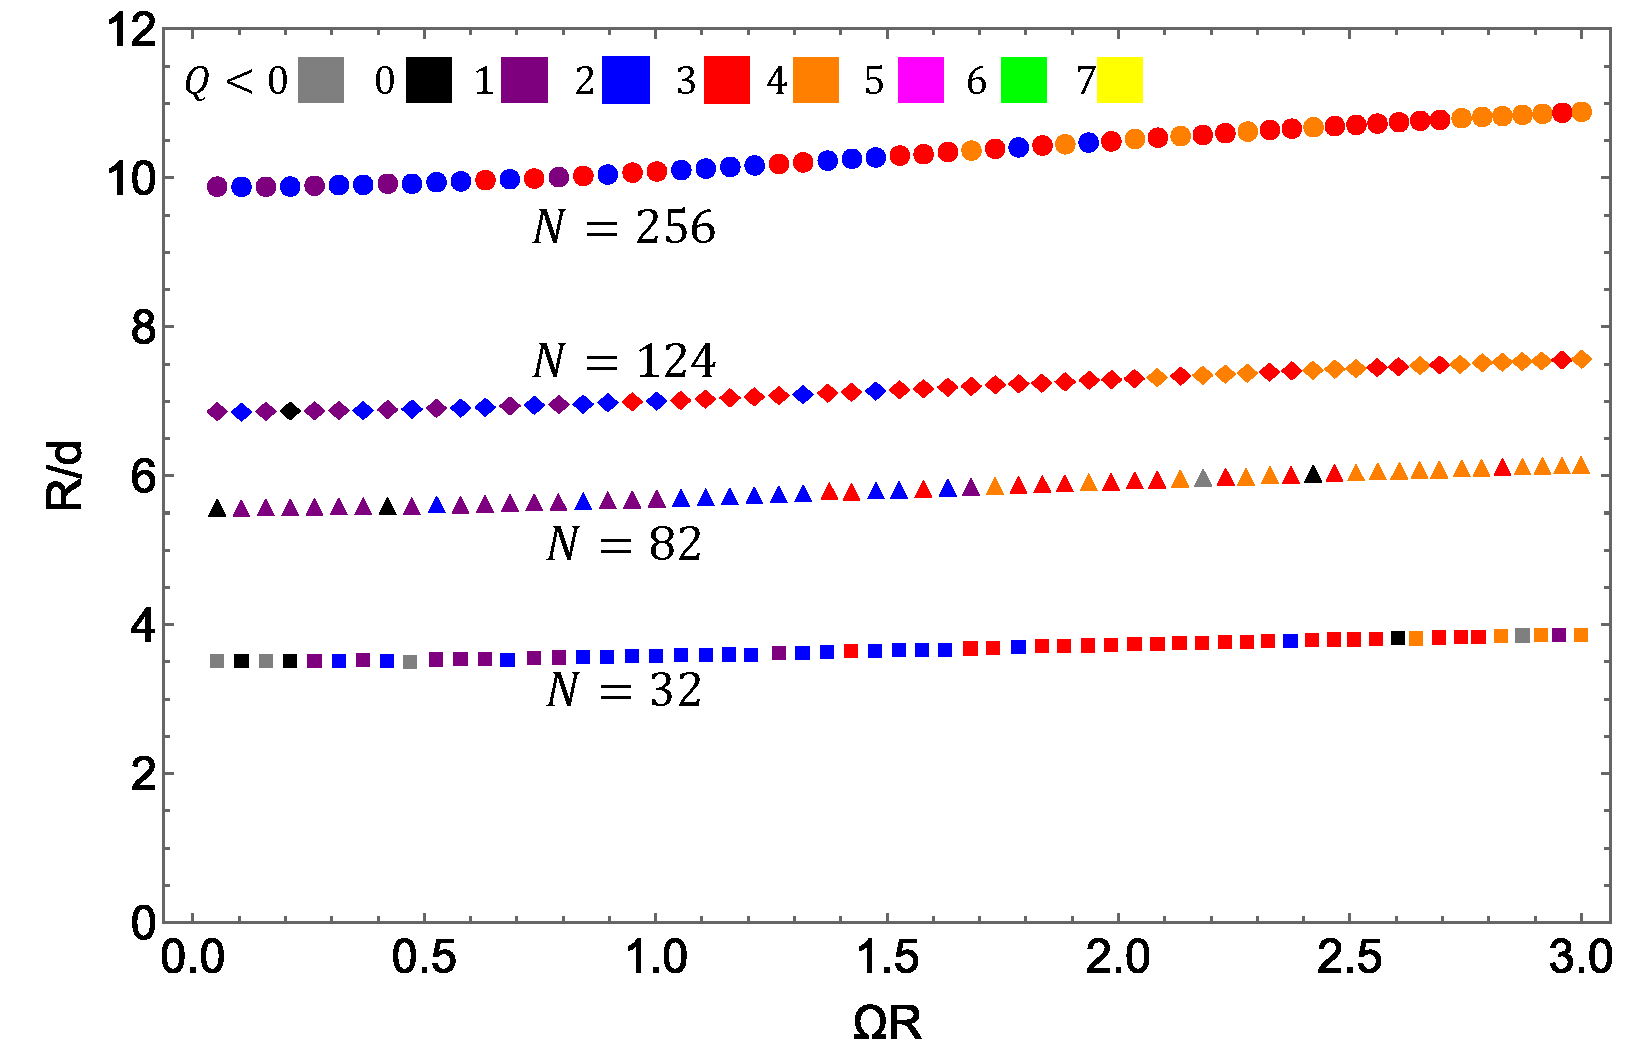
\includegraphics[width=1.0\linewidth]{mincounts_v4.pdf}
    \caption{Minimum topological charge $Q$ found for different $R/d$ vs. 
$\Omega R$ represented by a discrete color scale. While we vary $\Omega R$ over a similar range as in Ref.~\cite{bruss2012non}, we note that we only infrequently observe $Q=0$ (black markers), even in the low-twist regime. }
    \label{fig:minCharge} 
\end{figure}

In addition to the difficulty in finding \emph{minimally} defective ground states (i.e., states with $Q=0$ at low twist), we surprisingly find \emph{fewer} than expected defects for moderately large filament bundles.
Although this may be related to the difficulty in properly accounting for defect charge of boundary particles --- and hence may actually be reflective of states with much higher total charge --- this was nevertheless surprising.
As noted above, this boundary counting issue is almost certainly at play for small particle simulations (for which the boundary and boundary-neighbor particles make up a majority of the system), suggesting that our method may only recover the correct behavior for large $N$.
While our \emph{mean} charge counts seem to appropriately approach the limiting value of $Q=6$ expected of ground states at high $\Omega R$, we nevertheless find that even for minimizations of $N=256$ particles we typically find ``optimal'' ground states with smaller than expected $Q$.
We note that although the scale of spatial discretization we have chosen for these studies is reasonably small, we have not systematically checked the robustness of our defect counts to progressively refining the mesh.


\section{Discussion and future developments}\label{sec:conclusion}

We have a presented a new framework for simulating particles on curved surfaces. We build around existing exact geodesic solvers on discretized surfaces \cite{xin2009improving}, and implement new interfaces and data structures to efficiently submesh the surface when dealing with particles that interact via finite-range potentials. We integrate this with a standard, easily extensible object-oriented framework written in \CC{} to allow researchers to easily adapt our code with specialized particle-particle interactions or dynamical update rules appropriate to their system. We have provided standard reports for the scaling of our implementation -- at fixed or varying particle number, on meshes of fixed or varying complexity, and when parallelizing across multiple processors -- so that other researchers may easily estimate whether simulations of a particular use-case may be achieved. 

We have chosen a particular, MMP-like geodesic distance solver, but we note that there are interesting differences in the computational complexity of alternate choices -- such as the vector heat method \cite{sharp2019vector} -- and the way exact vs approximate solvers lead to different discretization errors. We are currently exploring the implementation of other approaches, something our object-oriented design makes straightforward. Given the potential importance of parallelizing the geodesic calculations, we are particularly interested in exploring the possibility of algorithms that will permit some of the geodesic calculations to be done on a GPU. 

Beyond this, natural extensions of our code base include the addition of vector-alignment interactions -- as  are common in models of flocking \cite{vicsek1995novel} -- to supplement the positional particle potentials already implemented. While we have so far focused on closed surfaces, it is well known that some interesting phenomena can only manifest themselves on surfaces with boundaries \cite{giomi2007crystalline}, for which we have looked at just one test case. Expansions of our work that explore and perhaps improve upon the existing boundary-handling routines --- including by implementing periodic boundary conditions --- may prove fruitful in the investigation of new problems.


The most up-to-date version of our codebase, including branches for our graphical user interface, other experimental future features, and a dedicated branch which allows the figures in this paper to be easily reproduced, can be found at \url{https://github.com/sussmanLab/curvedSpaceSim}.

\section{Acknowledgements}
We would like to thank Helen Ansell, Haicen Yue, and Tomilola Obadiya for fruitful discussions and critical comments on this manuscript. This material is based upon work supported by the National Science Foundation under Grant No.~DMR-2143815.
This research used the Delta advanced computing and data resource which is supported by the National Science Foundation (award OAC 2005572) and the State of Illinois. Delta is a joint effort of the University of Illinois Urbana-Champaign and its National Center for Supercomputing Applications.


%% The Appendices part is started with the command \appendix;
%% appendix sections are then done as normal sections
%% \appendix

%% \section{}
%% \label{}

%% References
%%
%% Following citation commands can be used in the body text:
%% Usage of \cite is as follows:
%%   \cite{key}         ==>>  [#]
%%   \cite[chap. 2]{key} ==>> [#, chap. 2]
%%

%% References with bibTeX database:

\bibliographystyle{elsarticle-num}
\bibliography{curvedSpaceSimulationsRefs}

%% Authors are advised to submit their bibtex database files. They are
%% requested to list a bibtex style file in the manuscript if they do
%% not want to use elsarticle-num.bst.

%% References without bibTeX database:

% \begin{thebibliography}{00}

%% \bibitem must have the following form:
%%   \bibitem{key}...
%%

% \bibitem{}

% \end{thebibliography}


\end{document}

%%
%% End of file 
